\documentclass{mynotes}

\usepackage{amsmath,amsfonts,amsthm,amssymb}
\usepackage{bm}
%\usepackage{indentfirst}
\usepackage{algorithm}
\usepackage{algpseudocode}

\usepackage{tikz}

\newtheorem{example}{Ví dụ}

\newcommand{\MC}{\mathcal{C}}
\newcommand{\FF}{\mathbb{F}}
\newcommand{\NN}{\mathbb{N}}
\newcommand{\ZZ}{\mathbb{Z}}
\newcommand{\RR}{\mathbb{R}}
\newcommand{\II}{\mathbb{I}}


\DeclareMathOperator{\Ima}{im}
\DeclareMathOperator{\tr}{tr}
\DeclareMathOperator{\rank}{rank}
\DeclareMathOperator{\sign}{sign}
\DeclareMathOperator{\spa}{spa}
\DeclareMathOperator{\sgn}{sgn}
\DeclareMathOperator{\lb}{label}

\setlength{\parskip}{4pt}
\addbibresource{references.bib}

\begin{document}

\tableofcontents

\chapter{Ma trận}

\section{Định thức của ma trận}

Trong các bài viết của mình thì vector sẽ được ký hiệu bởi chữ thường in đậm (ví dụ $\bm{v},\ \bm{x}, \cdots$)​; ma trận sẽ được ký hiệu bởi chữ hoa in đậm (ví dụ $\bm{A},\ \bm{B}, \cdots$​); các đại lượng vô hướng (số) được ký hiệu bởi chữ thường không in đậm (ví dụ $x_1,\ N,\ t, \cdots$).

Ví dụ vector $\bm{a} = (x_1, x_2, \cdots, x_n)$​ trong đó $x_i$​ là các tọa độ.

Ví dụ ma trận $\bm{A} = \begin{pmatrix}x_{11} & x_{12} & \cdots & x_{1n} \\ x_{21} & x_{22} & \cdots & x_{2n} \\ \cdots & \cdots & \cdots & \cdots \\ x_{n1} & x_{n2} & \cdots & x_{nn}\end{pmatrix}$.

\begin{definition}[Nghịch thế]
    Cho tập hợp $A = \{1, 2, \cdots, n\}$ và xét hoán vị $\sigma$ trên ​$A$. Ta gọi hai phần tử $i$​ và $j$​ tạo thành \textbf{nghịch thế} (inversion) nếu $i < j$​ và $\sigma(i) > \sigma(j)$.

    Đặt $\sigma = \{k_1, k_2, \cdots, k_n\}$​ là một hoán vị của $A$​. Ta ký hiệu \[ P\{k_1, k_2, \cdots, k_n\} \] là số lượng nghịch thế của $\sigma$​ và đặt \[ (-1)^{P\{k_1, k_2, \cdots, k_n\}} = \sign \{k_1, k_2, \cdots, k_n\}. \]
\end{definition}

Ví dụ với $n=4$​, $A = \{1, 2, 3, 4\}$​. Xét hoán vị $\sigma = \{4, 2, 1, 3\}$.

Ta nhận thấy các cặp nghịch thế $(4, 2),\ (4, 1),\ (4, 3),\ (2, 1)$​ gồm 4 cặp nghịch thế. Vậy $P\{4, 2, 1, 3\} = 4$ và $\sign \{4, 2, 1, 3\}=(-1)^4=1$​.

\begin{definition}[Định thức]
    Khi đó định thức của ma trận $\bm{A} = \begin{pmatrix}a_{11} & a_{12} & \cdots & a_{1n} \\ a_{21} & a_{22} & \cdots & a_{2n} \\ \cdots & \cdots & \cdots & \cdots \\ a_{n1} & a_{n2} & \cdots & a_{nn}\end{pmatrix}$ được định nghĩa là:
    \begin{equation}
        \det(\bm{A})=\displaystyle{\sum_{(i_1, i_2, \cdots, i_n)} a_{1, i_1} \cdot a_{2, i_2} \cdot a_{n, i_n} \cdot \sign\{i_1, i_2, \cdots, i_n\}}
    \end{equation}
    với mọi hoán vị $(i_1, i_2, \cdots, i_n)$ của $(1, 2, \cdots, n)$. Như vậy có $n!$​ phần tử cho tổng trên.
\end{definition}

Ví dụ: tính định thức ma trận $\bm{A}=\begin{pmatrix}1 & 2 & 3 \\ 4 & 5 & 6 \\ 7 & 8 & 9\end{pmatrix}$​.

Xét hoán vị $\sigma_1 = \{1, 2, 3\}$​. Khi đó $P\{1, 2, 3\}=0$​, $a_{11} \cdot a_{22} \cdot a_{33} \cdot (-1)^0 = 1 \cdot 5 \cdot 9 \cdot 1 = 45$​.

Xét hoán vị $\sigma_2 = \{1, 3, 2\}$​. Khi đó $P\{1, 3, 2\} = 1$​, $a_{11} \cdot a_{23} \cdot a_{32} \cdot (-1)^1 = 1 \cdot 6 \cdot 8 \cdot (-1) = -48$.

Xét hoán vị $\sigma_3 = \{2, 1, 3\}$​. Khi đó $P\{2,1,3\}=1$​, $a_{12} \cdot a_{21} \cdot a_{33} \cdot (-1)^1 = 2 \cdot 4 \cdot 9 \cdot (-1) = -72$.

Xét hoán vị $\sigma_4=\{2,3,1\}$. Khi đó $P\{2, 3, 1\} = 2$​, $a_{12} \cdot a_{23} \cdot a_{31} \cdot (-1)^2 = 2 \cdot 6 \cdot 7 \cdot 1 = 84$​.

Xét hoán vị $\sigma_5=\{3, 1, 2\}$. Khi đó $P\{3, 1, 2\} = 2$​, $a_{13} \cdot a_{21} \cdot a_{32} \cdot (-1)^2 = 3 \cdot 4 \cdot 8 \cdot 1 = 96$​.

Xét hoán vị $\sigma_6=\{3, 2, 1\}$​. Khi đó $P\{3, 2, 1\}=3$​, $a_{13} \cdot a_{22} \cdot a_{31} \cdot (-1)^3 = 3 \cdot 5 \cdot 7 \cdot  (-1) = -105$​.

Như vậy $\det(A)=45-48-72+84+96-105=0$​.

Định thức của ma trận còn được định nghĩa như sau:

Với ma trận $1 \times 1$ là $\bm{A}=\begin{pmatrix}a_{11}\end{pmatrix}$ thì $\det(\bm{A})=a_{11}$.

Với ma trận $2 \times 2$ là $\bm{A} = \begin{pmatrix}a_{11} & a_{12} \\ a_{21} & a_{22}\end{pmatrix}$​ thì $\det(\bm{A})=a_{11}a_{22} - a_{21}a_{12}$.

Với ma trận $n \times n$, gọi $\bm{M}_{ij}$ là ma trận có được từ ma trận $\bm{A}$ khi bỏ đi hàng $i$​ và cột $j$​ của ma trận $\bm{A}$ và ký hiệu $A_{ij}=(-1)^{i+j} \det (\bm{M}_{ij})$. Khi đó:

\begin{theorem}[Định lý Laplace]
    Định lý Laplace cho phép ta khai triển định thức của ma trận cấp $n$ thành tổng các ma trận cấp $n-1$.

    Khai triển theo cột $j$​: \[ \det(\bm{A})=\displaystyle{\sum_{i=1}^na_{ij} A_{ij}} = a_{1j} A_{1j} + a_{2j} A_{2j} + \cdots + a_{nj} A_{nj},\ j = \overline{1, n}.\]

    Khai triển theo hàng $i$​: \[ \det(\bm{A})=\displaystyle{\sum_{j=1}^n a_{ij} A_{ij}} = a_{i1} A_{i1} + a_{i2} A_{i2} + \cdots + a_{in} A_{in},\ i = \overline{1, n}. \]​
\end{theorem}

\section{Ma trận nghịch đảo}

Ma trận $\bm{A}^{-1}$​ được gọi là \textbf{ma trận nghịch đảo} của ma trận vuông $\bm{A}$ nếu $\bm{A}^{-1} \cdot \bm{A} = \bm{A} \cdot \bm{A}^{-1} = \bm{I}$​. Trong đó $\bm{I}$ là ma trận đơn vị cùng kích thước với $\bm{A}$.

\begin{equation}
    \bm{A}^{-1}=\frac{1}{\det(\bm{A})}[(A_{ij})_n]^T=\frac{1}{\det(\bm{A})}\begin{pmatrix} A_{11} & A_{21} & \cdots & A_{n1} \\ A_{12} & A_{22} & \cdots & A_{n2} \\ \cdots & \cdots & \cdots & \cdots \\ A_{1n} & A_{2n} & \cdots & A_{nn} \end{pmatrix}
\end{equation}

Như vậy, điều kiện cần và đủ để một ma trận có nghịch đảo là định thức khác 0.

\section{Hạng của ma trận}

\begin{definition}[Hạng của ma trận]
    Cho ma trận $\mathbf{A}_{m \times n}$. \textbf{Hạng} của ma trận là cấp của ma trận con lớn nhất có định thức khác 0. Nghĩa là một ma trận vuông mà là ma trận con (lấy 1 phần của ma trận gốc) kích thước $r \times r$ mà có định thức khác 0, thì hạng của ma trận khi đó là $r$. Dễ thấy do là ma trận con, và vuông, nên $r \leqslant \min(m, n)$.
\end{definition}

Ví dụ, ma trận $\bm{A} = \begin{pmatrix}1 & 2 & 3 \\ 2 & 4 & 6 \\ 1 & 2 & 4\end{pmatrix}$ có định thức $\det(\bm{A}) = 0$. Nhưng ma trận con của $\bm{A}$ là $\bm{B} = \begin{pmatrix}2 & 3 \\ 2 & 4\end{pmatrix}$ (lấy dòng 1 và 3, lấy cột 2 và 3) có định thức $\det(\bm{B}) = 2 \neq 0$, do đó $r = \text{rank}(\bm{A}) = 2$ ($\text{rank}(\bm{A})$ nghĩa là hạng của $\bm{A}$).

\chapter{Discrete logarithm}

\section{Các thuật toán tính discrete logarithm}

Thuật toán Baby-Step-Giant-Step (BSGS) giúp tính discrete logarithm trên nhóm cyclic với order là số nguyên tố \ref{alg:bsgs}.

\begin{algorithm}[H]
    \caption{Thuật toán Baby-Step-Giant-Step}
    \label{alg:bsgs}
    \begin{algorithmic}[1]
        \Require Nhóm cyclic $G$ có order $n$, generator $g$ và phần tử $h \in G$.
        \Ensure Số $x$ duy nhất thuộc $\{ 0, 1, \ldots, n-1 \}$ thỏa $g^x = h$.
        $m \gets \lfloor \sqrt{n} \rfloor$
        \For{$j = 0 \to m-1$}
            \State Tính $g^j$. Lưu $(j, g^j)$ vào bảng.
        \EndFor
        \State Tính $g^{-m}$.
        \State $\gamma \gets h$.
        \For{$i = 0 \to m-1$}
            \State a) Kiểm tra điều kiện $\gamma = g^j$ với $j = 0, 1, \ldots, m-1$.
            \State b) Nếu điều kiện thỏa, trả về $im + j$.
            \State c) Nếu không, đặt $\gamma \gets \gamma \cdot g^{-m}$.
        \EndFor
    \end{algorithmic}
\end{algorithm}

Khi order của cyclic group là lũy thừa một số nguyên tố thì ta dùng thuật toán Pohlig-Hellman \ref{alg:pohlig}.

\begin{algorithm}[H]
    \caption{Thuật toán Pohlig-Hellman}
    \label{alg:pohlig}
    \begin{algorithmic}[1]
        \Require Nhóm cyclic $G$ có order $n=p^e$, generator $g$ và phần tử $h \in G$.
        \Ensure Số $x$ duy nhất thuộc $\{ 0, 1, \ldots, n-1 \}$ thỏa $g^x = h$.
        \State Khởi tạo $x_0 = 0$.
        \State Tính $\gamma = g^{p^{e-1}}$. Theo định lý Lagrange, $\gamma$ có order là $p$.
        \For{$k = 0 \to e-1$}
            \State a) Tính $h_k = (g^{-x_k} \cdot h)^{e-1-k}$.
            \State b) Sử dụng thuật toán baby-step-giant-step, tìm $d_k \in \{ 0, 1, \ldots, p-1 \}$ sao cho $\gamma^{d_k} = h_k$. % Bước này có độ phức tạp $O(\sqrt{p})$.
            \State c) Tính $x_{k+1} = x_k + p^k d_k$.
        \EndFor
        \State Trả về $x_e$ là kết quả cần tìm.
    \end{algorithmic}
\end{algorithm}

\chapter{Số học}

\section{Thặng dư chính phương}

\begin{definition}[Số chính phương modulo $p$]
    Xét số dương nguyên tố lẻ $p$. Số $a$ được gọi là \textbf{số chính phương modulo $p$} nếu $(a, m) = 1$ và tồn tại số $x$ sao cho $x^2 = a \pmod p$.

    Nói cách khác phương trình đồng dư $x^2 \equiv a \pmod p$ có nghiệm.
\end{definition}

Chúng ta sử dụng kí hiệu Legendre (Legendre's symbol) để thể hiện một số $a$ có phải là số chính phương modulo nguyên tố $p$ không.

\begin{definition}[Legendre's symbol]
    Xét $p$ là số nguyên tố, $a$ là số nguyên không chia hết cho $p$. Khi đó kí hiệu Legendre được định nghĩa là
    \begin{equation}
        \left(\frac{a}{p}\right) = \begin{cases}
            1, & \text{ nếu } a \text{ là số chính phương modulo } p. \\
            -1, & \text{ nếu ngược lại.}
        \end{cases}
    \end{equation}
\end{definition}

\chapter{Lattice-based crypto}

\section{Thuật toán GGH}

Phần này tham khảo trong \cite{HofJef-2014}

Trong thuật toán GGH, ta chọn số nguyên tố $q$ làm public parameter.

Sau đó chọn hai số $f$ và $g$ làm secret key. Hai số này phải thỏa mãn các điều kiện \[ f < \sqrt{q/2}, \quad \sqrt{q/4} < g < \sqrt{q/2}, \quad \gcd(f, qg) = 1 \]

Tính $h = f^{-1} g \pmod q$. Khi đó public key là $h$.

\textbf{Encryption}. Để encrypt message $m$ với số random $r$ thỏa mãn \[ 0 < m < \sqrt{q/4}, \quad 0 < r < \sqrt{q/2} \]

Ta tính $e = rh + m \pmod q$ là ciphertext với $0 < e < q$.

\textbf{Decryption}. Để decrypt ciphertext $e$ ta tính \[ a = fe \pmod q, \quad b = f^{-1} a \pmod g \]

Lưu ý $f^{-1}$ là nghịch đảo modulo $g$. Khi đó $b \equiv m$ là message ban đầu.

\begin{proof}
    Để chứng minh rằng số $b$ sau khi tính toán bằng chính xác $m$ ban đầu ta cần xem xét điều kiện của secret key và public key.

    Đầu tiên ta có \[ a \equiv fe \equiv f(rh + m) = f(r f^{-1} g + m) = rg + fm \pmod q \]

    Từ điều kiện của $f$, $g$, $r$ và $m$ ta có \[ rg + fm < \sqrt{\dfrac{q}{2}} \cdot \sqrt{\dfrac{q}{2}} + \sqrt{\dfrac{q}{2}} \cdot \sqrt{\dfrac{q}{4}} < q \]

    Nói cách khác $rg + fm$ giữ nguyên giá trị trong phép modulo $q$, hay $a \equiv rg + fm$.

    Suy ra $b = f^{-1} a = f^{-1} (rg + fm) = m \pmod g$ (giá trị $a$ không thay đổi khi chuyển từ modulo $q$ sang modulo $g$). Do $0 < m < \sqrt{q/4}$ và $\sqrt{q/4} < g < \sqrt{q/2}$ nên $m < g$. Nói cách khác $b$ bằng đúng $m$ ban đầu.
\end{proof}

Để tấn công hệ mật mã này ta xây dựng lattice. Để ý rằng $h = f^{-1} g \pmod q$, hay $fh + kq = g$ với $k \in \ZZ$.

Ta thấy rằng $f \cdot (h, 1) + k \cdot (q, 0) = (g, f)$. Như vậy lattice gồm hai vector $(h, 1)$ và $(q, 0)$. Thuật toán tối giản Gauss sẽ hoạt động trong trường hợp này (số chiều bằng 2).

\chapter{Bài toán đếm Polya}

\section{Lớp tương đương}

Xét nhóm $G$ và tập hợp $M$. Khi đó hai phần tử $m$ và $n$ thuộc $M$ được gọi là \textbf{quan hệ với nhau} nếu tồn tại $g \in G$ mà $m = g n$.

\begin{remark}
    Quan hệ giữa các phần tử như trên là quan hệ tương đương.    
\end{remark}


\begin{proof}
    Để chứng minh một quan hệ là tương đương, ta cần chứng minh tính phản xạ, đối xứng và bắc cầu.

    Đối với tính phản xạ, mọi vector đều có quan hệ với chính nó qua phần tử đơn vị $e \in G$.

    Đối với tính đối xứng, nếu $m$ có quan hệ với $n$ thì tồn tại $g \in G$ sao cho $m = gn$. Theo tính chất nhóm thì tồn tại phần tử $g^{-1}$ là nghịch đảo của $g$ trong $G$. Do đó $g^{-1} m = n$. Nói cách khác $n$ cũng có quan hệ với $m$. Như vậy ta có tính đối xứng.

    Đối với tính bắc cầu, nếu $m$ có quan hệ với $n$ thì tồn tại $g_1 \in G$ sao cho $m = g_1 n$. Tiếp theo, nếu $n$ có quan hệ với $p$ thì tồn tại $g_2 \in G$ sao cho $n = g_2 p$. Suy ra $m = g_1 n = g_1 (g_2 p) = (g_1 g_2) p$. Do $g_1, g_2 \in G$ nên $g_1 g_2 \in G$. Như vậy $m$ cũng có quan hệ với $p$ nên quan hệ có tính bắc cầu.

    Vậy quan hệ được định nghĩa như trên là quan hệ tương đương.
\end{proof}

\section{Tác động nhóm lên vector}

Xét nhóm $G$ và không gian vector $\FF_2^n$, $n \in \NN$. Khi đó hai vector $\bm{x}$ và $\bm{y}$ thuộc $\FF_2^n$ được gọi là \textbf{quan hệ với nhau} nếu tồn tại $g \in G$ mà $\bm{x} = g \bm{y}$.

Ví dụ, xét nhóm hoán vị $\mathcal{S}_3$. Giả sử các vector trong $\FF_2^3$ có dạng \[ \bm{x} = (x_1, x_2, x_3) \in \FF_2^3. \] 

Khi đó vector $(1, 0, 0)$ có quan hệ với $(0, 0, 1)$ với hoán vị $(1, 3)(2)$. Cụ thể là $(x_1, x_2, x_3) \xrightarrow{(1, 3)(2)} (x_3, x_2, x_1)$.

Tương tự, vector $(1, 0, 0)$ cũng có quan hệ với $(0, 1, 0)$ với hoán vị $(1, 2)(3)$. Thêm nữa, vector $(1, 0, 0)$ có quan hệ với chính nó qua hoán vị đồng nhất $(1)(2)(3)$.

Trong môn toán rời rạc ta đã biết, nếu một tập có quan hệ tương đương thì ta có thể phân các phần tử của tập đó vào các lớp tương đương rời nhau. Nghĩa là nếu hai phần tử có quan hệ với nhau thì vào cùng một lớp tương đương. Từ phần trên ta đã biết rằng dưới tác động của nhóm, các phần tử trong tập hợp bất kì sẽ phân bổ thành các lớp tương đương.

Câu hỏi đặt ra là, có bao nhiêu lớp tương đương như vậy?

Để giải quyết vấn đề này ta sử dụng bổ đề Burnside.

Nhóm $\mathcal{S}_3$ có các hoán vị \[ \mathcal{S}_3 = \{ (1)(2)(3), (1, 2)(3), (1, 3)(2), (2, 3)(1), (1, 3, 2), (1, 2, 3) \} \]

Lần lượt xét từng hoán vị. Đầu tiên, với $(1)(2)(3)$ thì các phần tử trong vector đứng yên. Do đó dưới tác động của hoán vị này, $x_1$ biến thành $x_1$, $x_2$ biến thành $x_2$ và $x_3$ biến thành $x_3$. Số cách chọn cho mỗi $x_i$ là 2 nên theo quy tắc nhân ta có $2^3 = 8$ cách.

Tiếp theo, với hoán vị $(1, 2)(3)$ thì $x_1 \to x_2$, $x_2 \to x_1$ và $x_3 \to x_3$. Do đó $x_1$ và $x_2$ có cùng giá trị nên có 2 cách chọn, $x_3$ cũng có 2 cách chọn nên tổng số cách là $2 \cdot 2 = 4$. Hoán vị $(1, 3)(2)$ và $(2, 3)(1)$ tương tự.

Với hoán vị $(1, 2, 3)$ thì $x_1 \to x_2$, $x_2 \to x_3$ và $x_3 \to x_1$ nên $x_1 = x_2 = x_3$, có 2 cách chọn trong trường hợp này. Hoán vị $(1, 3, 2)$ tương tự.

Như vậy, theo bổ đề Burnside, số lớp tương đương các vector trong $\FF_2^3$ là \[ t(\mathcal{S}_3) = \frac{1}{6} (1 \cdot 2^3 + 3 \cdot 2^2 + 2 \cdot 2) = 4 \]

Thật vậy, ta có thể chia các vector thành 4 lớp tương đương là $\{ 000 \}$, $\{ 001, 010, 011 \}$, $\{ 011, 101, 110 \}$, $\{ 111 \}$.

Ngoài nhóm $\mathcal{S}_3$ ra còn các nhóm khác cũng tác động lên các vector. Một số nhóm hay được sử dụng là:

\begin{enumerate}
    \item Nhóm general linear: gồm các ma trận khả nghịch $n \times n$ trên $\FF_2$. Tác động nhóm lúc này là phép nhân ma trận $\bm{A} \in GL(n, 2)$ với vector $\bm{x} \in \FF_2^n$, hay $\bm{A} \cdot \bm{x}$.
    \item Nhóm general affine: gồm các ma trận khả nghịch $n \times n$ trên $\FF_2$ và vector bất kì trong $\FF_2^n$. Tác động nhóm lúc này là biến đổi affine $\bm{A} \cdot \bm{x} + \bm{b}$ với $\bm{A} \in GL(n, 2)$ và $\bm{b} \in \FF_2^n$.
\end{enumerate}

Cần nhắc lại một chút, số lượng phần tử của nhóm $GL(n, 2)$ là \[ (2^n - 1) \cdot (2^n - 2) \cdots (2^n - 2^{n-1}) \]

Khi $n = 3$ thì $\lvert GL(3, 2) \rvert = (2^3 - 1) \cdot (2^3 - 2) \cdot (2^3 - 4) = 168$ ma trận.

\section{Tác động nhóm lên hàm boolean}

Ta tiếp tục xét nhóm $G$ và không gian vector $\FF_2^n$, $n \in \NN$. Khi đó hai hàm boolean $n$ biến $f(x_1, \ldots, x_n)$ và $g(x_1, \ldots, x_n)$ được gọi là \textbf{quan hệ với nhau} nếu tồn tại $g \in G$ mà $g(\bm{x}) = f(g \bm{x})$ với mọi $\bm{x} \in \FF_2^n$.

Ta cũng xét hoán vị $\mathcal{S}_3$. Ta cũng lần lượt xét các phần tử của nhóm.

Đặt $f_0, f_1, \ldots, f_7$ lần lượt là các giá trị hàm $f$ với các vector $\bm{x} \in \FF_2^3$.

Đầu tiên, với $(1)(2)(3)$, ta có bảng chuyển vector như sau

\begin{figure}[ht]
    \centering
    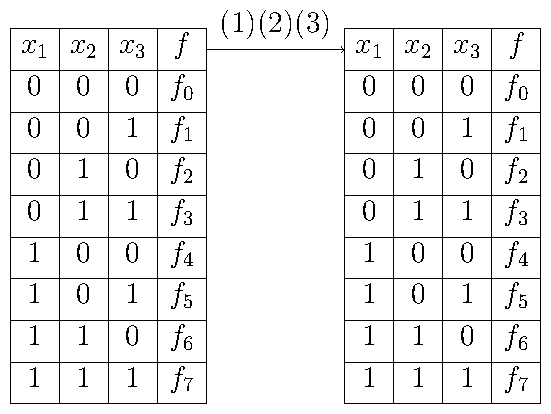
\includegraphics{./mynotes-figures/bool1.pdf}
\end{figure}

Ta thấy rằng $f_0 \to f_0$, $f_1 \to f_1$, ..., $f_7 \to f_7$ nên có 8 chu trình. Vậy số lượng cách chọn là $2^8$.

Tiếp theo, xét các hoán vị dạng $(1)(2, 3)$, ta có bảng chuyển vector như sau

\begin{figure}[ht]
    \centering
    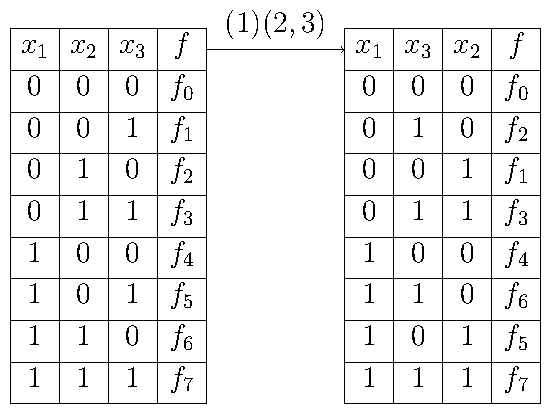
\includegraphics{./mynotes-figures/book2.pdf}
\end{figure}

Ta thấy rằng $f_0 \to f_0$, $f_1 \to f_2 \to f_1$, $f_3 \to f_3$, $f_4 \to f_4$, $f_5 \to f_6 \to f_5$, $f_7 \to f_7$. Ở đây có 6 chu trình nên số cách chọn là $2^6$.

Tiếp theo ta xét các hoán vị dạng $(1, 2, 3)$.

\begin{figure}[ht]
    \centering
    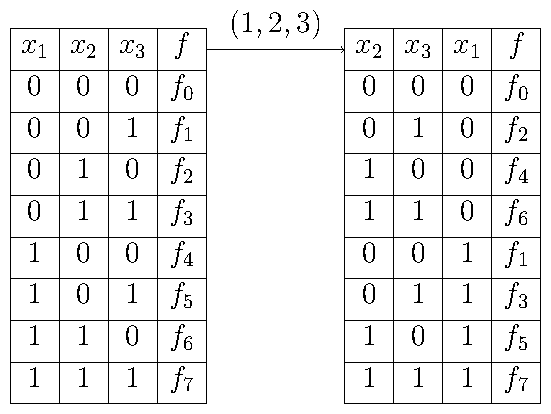
\includegraphics{./mynotes-figures/book3.pdf}
\end{figure}

Ta thấy rằng $f_0 \to f_0$, $f_1 \to f_2 \to f_4 \to f_1$, $f_3 \to f_6 \to f_5 \to f_3$, $f_7 \to f_7$ nên ở đây có 4 chu trình. Số cách chọn là $2^4$.

Như vậy theo bổ đề Burnside, số lớp hàm bool tương đương dưới tác động của nhóm $\mathcal{S}_3$ là \[ t (\mathcal{S}_3) = \dfrac{1}{6}(2^8 + 3 \cdot 2^6 + 2 \cdot 2^4) = 80. \]

\chapter{Giải tích}

\begin{definition}[Dãy Cauchy]
    Dãy $(x_n)$ được gọi là dãy Cauchy nếu với mọi $\varepsilon > 0$, tồn tại $N_0 \in \NN$ sao cho, với mọi $m, n > N_0$ thì $\lvert x_m - x_n \rvert < \varepsilon$.
\end{definition}

\begin{theorem}[Tiêu chuẩn Cauchy]
    Dãy số $(x_n)$ có giới hạn hữu hạn khi và chỉ khi nó là dãy Cauchy.
\end{theorem}

\begin{theorem}[Bổ đề Fermat]
    Cho $f$ là một hàm số có đạo hàm trên $(a, b)$. Nếu $x_0 \in (a, b)$ là một điểm cực trị của $f$ thì ta có $f'(x_0) = 0$.
\end{theorem}

\begin{proof}
    Ta chứng minh trong trường hợp $x_0$ là điểm cực tiểu. Trường hợp điểm cực đại tương tự.

    Hàm $f$ có đạo hàm trên $(a, b)$ nên tại điểm $x_0$ nó có đạo hàm bên trái và đạo hàm bên phải, và hai đạo hàm này bằng nhau.

    Ta có $\displaystyle{f'(x_0^+) = \lim_{x \to x_0^+} \frac{f(x) - f(x_0)}{x - x_0}}$. Vì $x \to x_0^+$ nghĩa là $x > x_0$ ($x$ tiến tới $x_0$ từ bên phải), và do $x_0$ là cực tiểu $f(x) - f(x_0) \geqslant 0$ nên phân số dưới dấu giới hạn lớn hơn 0. Suy ra $f'(x_0^+) \geqslant 0$.

    Hoàn toàn tương tự ta chứng minh được $f'(x_0^-) \leqslant 0$. Và do $f'(x_0^+) = f'(x_0^-) = f'(x_0)$ nên $f'(x_0) = 0$.

    Ta có điều phải chứng minh.
\end{proof}

\begin{theorem}[Định lí Rolle]
    Xét hàm số $f$ liên tục trên đoạn $[a, b]$, có đạo hàm trên khoảng $(a, b)$ và $f(a) = f(b)$. Khi đó tồn tại $c$ thuộc $(a, b)$ sao cho $f'(c) = 0$.
\end{theorem}

\begin{theorem}[Định lí Lagrange]
    Xét hàm số $f$ liên tục trên đoạn $[a, b]$, có đạo hàm trên khoảng $(a, b)$. Khi đó tồn tại $c$ thuộc $(a, b)$ sao cho $f'(c) (b - a) = f(b) - f(a)$.
\end{theorem}

\begin{definition}[Hàm lõm]
    Hàm số $f$ liên tục trên khoảng $\II$ nếu với mọi $\alpha, \beta$ mà $\alpha + \beta = 1$ ta đều có 
    \begin{equation}
        f(\alpha x + \beta y) \leqslant \alpha f(x) + \beta f(y), \quad \forall x, y \in \II
    \end{equation}
\end{definition}

\chapter{Quantum computing}

\section{Introduction}

Toán tử $NOT$ được biểu diễn dưới dạng ma trận $\begin{pmatrix}
    0 & 1 \\ 1 & 0
\end{pmatrix}$. Khi đó $NOT(\alpha \lvert 0 \rangle + \beta \lvert 1 \rangle) = \beta \lvert 0 \rangle + \alpha \lvert 1 \rangle$.

Nếu cho $\alpha = \beta = 1$ và $x \in \{0, 1\}$ thì $NOT \lvert x \rangle = \lvert x \oplus 1 \rangle$.

Toán tử Hadarmard được biểu diễn dưới dạng ma trận \[ \mathcal{H} = \frac{1}{\sqrt{2}} \begin{pmatrix}
    1 & 1 \\ 1 & -1
\end{pmatrix} \]

Khi đó \[ \mathcal{H} (\alpha \lvert 0 \rangle + \beta \lvert 1 \rangle) = \frac{1}{\sqrt{2}} \begin{pmatrix}
    1 & 1 \\ 1 & - 1
\end{pmatrix} \begin{pmatrix}
    \alpha \\ \beta
\end{pmatrix} = \frac{1}{\sqrt{2}} \begin{pmatrix}
    \alpha + \beta \\ \alpha - \beta
\end{pmatrix} = \frac{\alpha + \beta}{\sqrt{2}} \lvert 0 \rangle + \frac{\alpha - \beta}{\sqrt{2}} \lvert 1 \rangle \]

Nếu $\alpha = 1, \beta = 0$ thì $\mathcal{H} (\lvert 0 \rangle) = \dfrac{1}{\sqrt{2}} \lvert 0 \rangle + \dfrac{1}{\sqrt{2}} \lvert 1 \rangle$.

Nếu $\alpha = 0, \beta = 1$ thì $\mathcal{H} (\lvert 1 \rangle) = \dfrac{1}{\sqrt{2}} \lvert 0 \rangle + \dfrac{-1}{\sqrt{2}} \lvert 1 \rangle$.

Tổng hợp lại, nếu $x \in \{0, 1\}$ thì $\mathcal{H} \lvert x \rangle = \dfrac{1}{\sqrt{2}} \lvert 0 \rangle + \dfrac{(-1)^x}{\sqrt{2}} \lvert 1 \rangle$.

Ta thấy rằng toán tử ngược của toán tử Hadamard là chính nó.

Đố vui: nếu ta có qubit là $\alpha \lvert 0 \rangle + \beta \lvert 1 \rangle$, hãy xây dựng mạch logic để biến đổi qubit trên thành $\alpha \lvert 000 \rangle + \beta \lvert 111 \rangle$.

Giải: sử dụng toán tử Hadamard và NOT. Ta có \[ NOT(\alpha \lvert 0 \rangle + \beta \lvert 1 \rangle) = \beta \lvert 0 \rangle + \alpha \lvert 1 \rangle\] và \[\mathcal{H} (\alpha \lvert 0 \rangle + \beta \lvert 1 \rangle) = \dfrac{1}{\sqrt{2}} (\alpha + \beta) \lvert 0 \rangle + \dfrac{1}{\sqrt{2}} (\alpha - \beta) \lvert 1 \rangle \]

Toán tử $CNOT$ được biểu diễn bởi ma trận \[ CNOT = \begin{pmatrix}
    1 & 0 & 0 & 0 \\ 0 & 1 & 0 & 0 \\ 0 & 0 & 0 & 1 \\ 0 & 0 & 1 & 0
\end{pmatrix}\]

Giả sử ta có hai qubit là $\lvert \alpha \rangle = x \lvert 0 \rangle + y \lvert 1 \rangle$ và $\lvert \beta \rangle = z \lvert 0 \rangle + t \lvert 1 \rangle$.

Khi đó $\lvert \alpha \rangle \otimes \lvert \beta \rangle = xz \lvert 00 \rangle + xt \lvert 01 \rangle + yz \lvert 10 \rangle + yt \lvert 11 \rangle$.

Qua toán tử $CNOT$ ta có

\begin{align*}
    CNOT (\lvert \alpha \rangle \otimes \lvert \beta \rangle) 
    = & \begin{pmatrix}
    1 & 0 & 0 & 0 \\ 0 & 1 & 0 & 0 \\ 0 & 0 & 0 & 1 \\ 0 & 0 & 1 & 0
    \end{pmatrix} \begin{pmatrix}
    xz \\ xt \\ yz \\ yt
    \end{pmatrix}
    = \begin{pmatrix}
    xz \\ xt \\ yt \\ yz
    \end{pmatrix} \\
    = & xz \lvert 00 \rangle + xt \lvert 01 \rangle + yt \lvert 10 \rangle + yz \lvert 11 \rangle
\end{align*}

Trường hợp $\lvert \alpha \rangle = \lvert 0 \rangle$ thì $x = 1, y = 0$. Khi đó ta có tương đương \[ CNOT (\lvert 0 \rangle \otimes \lvert \beta \rangle) = z \lvert 00 \rangle + t \lvert 01 \rangle = \lvert 0 \rangle \otimes (z \lvert 0 \rangle + t \lvert 1 \rangle) = \lvert 0 \rangle \otimes \lvert \beta \rangle. \]

Trường hợp $\lvert \alpha \rangle = \lvert 1 \rangle$ thì $x = 0, y = 1$. Khi đó ta có tương đương \[ CNOT (\lvert 1 \rangle) \otimes \lvert \beta \rangle) = t \lvert 10 \rangle + z \lvert 11 \rangle = \lvert 1 \rangle \otimes (t \lvert 0 \rangle + z \lvert 1 \rangle) = \lvert 1 \rangle \otimes NOT(\lvert \beta \rangle). \]

Nói cách khác, nếu $x \in \{0, 1\}$ thì \[ CNOT (\lvert x \rangle \otimes \lvert \beta \rangle) = \begin{cases}
    \lvert x \rangle \otimes \lvert \beta \rangle, & \text{nếu } x = 0 \\ \lvert x \rangle \otimes NOT(\lvert \beta \rangle), & \text{nếu } x = 1
\end{cases} \]

Do đó các toán tử có ma trận $\begin{pmatrix}
    I_n & \mathcal{O} \\ \mathcal{O} & \mathcal{U}
\end{pmatrix}$ được gọi là toán tử kiểm soát (controlled).

Một trường hợp riêng nữa là khi $\beta = 0$ hoặc $\beta = 1$. Khi đó, với toán tử $NOT$ bên trên ta suy ra \[ CNOT (\lvert x \rangle \otimes \lvert y \rangle) = \lvert x \rangle \otimes \lvert x \oplus y \rangle \]


\chapter{Lý thuyết xác suất}

\section{Định nghĩa xác suất}

\begin{definition}[Định nghĩa cổ điển của xác suất]
    Định nghĩa thống kê của xác suất nói rằng, giả sử trong một phép thử có $n$ khả năng có thể xảy ra. Xét một biến cố $A$ xảy ra khi thực hiện phép thử có $k$ khả năng xảy ra. Khi đó xác suất của biến cố $A$ ký hiệu là $P(A)$ và được tính \[P(A) = \frac{k}{n}\]
\end{definition}

Dễ thấy, do biến cố $A$ là một trường hợp nhỏ trong tổng thể tất cả trường hợp khi thực hiện phép thử, do đó $0 \leq k \leq n$. Nghĩa là \[0 \leq P(A) \leq 1\] với mọi biến cố $A$ bất kì.

\begin{example}
    Xét phép thử tung hai đồng xu. Gọi $A$ là biến cố hai đồng xu cùng mặt.
    
    Ta ký hiệu $S$ là đồng xu sấp, $N$ là đồng xu ngửa. Khi đó các trường hợp có thể xảy ra của phép thử là $S-S$, $S-N$, $N-S$, $N-N$ (4 trường hợp). 
    
    Trong khi đó, các trường hợp có thể xảy ra của biến cố $A$ là $S-S$, $N-N$ (2 trường hợp).
    
    Kết luận: $P(A) = \frac{2}{4} = \frac{1}{2}$
    
    Chúng ta gọi tập hợp tất cả các trường hợp khi thực hiện phép thử là \textbf{không gian mẫu} và ký hiệu là $\Omega$. Mỗi phần tử trong không gian mẫu được gọi là \textbf{biến cố sơ cấp}. Trong bài này, $\Omega = \{S-S, S-N, N-S, N-N\}$.
    
    Tập hợp các trường hợp có thể xảy ra của biến cố gọi là \textbf{không gian biến cố} và ký hiệu là $\Omega_A$. Trong bài này $\Omega_A = \{S-S, N-N\}$.
    
    Như vậy, $P(A) = \frac{|\Omega_A|}{|\Omega|}$
\end{example}

\begin{example}
    Tung hai con súc sắc cân đối và đồng chất. Tính xác suất tổng số nút của hai con súc sắc bằng 4.
    
    Việc tung mỗi con súc sắc có 6 trường hợp. Do đó $|\Omega| = 6^2 = 36$
    
    Gọi $A$ là biến cố tổng số nút của hai con súc sắc bằng 4. Ta có các trường hợp là $4=1+3=3+1=2+2$ (3 trường hợp).
    
    Như vậy $|\Omega_A| = 3$ và $P(A) = \frac{3}{36} = \frac{1}{12}$
\end{example}

\begin{definition}[Biến cố xung khắc]
    Hai biến cố được gọi là \textbf{xung khắc} nếu biến cố này xảy ra thì biến cố kia chắc chắn không xảy ra. Nói cách khác giao của chúng bằng rỗng.
\end{definition}
    
Khi đó, nếu $A$ và $B$ là hai biến cố xung khắc, \[P(A + B) = P(A) + P(B)\]
    
Ta còn có thể ký hiệu $P(A+B)$ là $P(A \cup B)$ (hợp hai biến cố).
    
\begin{definition}[Biến cố độc lập]
    Hai biến cố được gọi là \textbf{độc lập} nếu việc xảy ra của biến cố này không ảnh hưởng đến việc xảy ra của biến cố kia. 
\end{definition}

Khi đó, nếu $A$ và $B$ là hai biến cố độc lập thì \[P(AB) = P(A)P(B)\]    

\section{Xác suất có điều kiện}

Xét hai tập hợp $A$ và $B$. Số phần tử của phép hợp hai tập hợp trong trường hợp tổng quát được tính như sau: \[|A \cup B| = |A| + |B| - |A \cap B|\]
    
Tương tự, xác suất của phép cộng xác suất đối với hai biến cố có giao khác rỗng là: \[P(A + B) = P(A) + P(B) - P(A \cap B)\]

Xét các tập hợp $A_1$, $A_2$, ..., $A_n$. Khi đó, số phần tử khi hợp các tập hợp này là:
\begin{equation*}
    \begin{split}
        |A_1 \cup A_2 \cup \cdots \cup A_n| & = |A_1| + |A_2| + \cdots + |A_n| - \sum_{i, j}|A_i \cap A_j| \\ & + \sum_{i, j, k} |A_i \cap A_j \cap A_k| + \cdots \\ & = \sum_{i=1}^n (-1)^{i+1} \sum_{j_1, j_2, \cdots, j_i} |A_{j_1} \cap A_{j_2} \cap \cdots \cap A_{j_i} |
    \end{split}
\end{equation*}

Tương tự, ta có phép cộng xác suất:

\begin{theorem}[Phép cộng xác suất mở rộng]
    \begin{equation*}
        P(A_1 \cup A_2 \cup \cdots \cup A_n) = \sum_{i=1}^n (-1)^{i+1} \sum_{j_1, j_2, \cdots, j_i} P(A_{j_1} \cap A_{j_2} \cap \cdots \cap A_{j_i})
    \end{equation*}
\end{theorem}

\begin{theorem}[Xác suất có điều kiện]
    Xét hai biến cố $A$ và $B$. Khi đó xác suất xảy ra của biến cố $B$ với điều kiện biến cố $A$ xảy ra là: 
    \begin{equation}
        P(B | A) = \frac{P(AB)}{P(A)}
    \end{equation}
    Lúc này, $A$ và $B$ không độc lập.
\end{theorem}

Tổng quát, nếu $n$ biến cố $A_i$, $i=1, \ldots, n$ không độc lập thì:
\begin{align*}
    P(A_1 A_2 \cdots A_n) = & P(A_1) \cdot P(A_2|A_1) \cdot P(A_3 | A_2A_1) \cdots \\ & P(A_n|A_1A_2 \cdots A_{n-1})
\end{align*}

\begin{example}
    Xét hai câu hỏi trắc nghiệm có 4 lựa chọn. Tính xác suất học sinh trả lời đúng câu thứ hai với điều kiện câu đầu trả lời sai.
    
    \textbf{Giải}. Gọi $A$ là biến cố câu đầu tiên học sinh trả lời sai. $P(A) = \frac{3}{4}$
    
    Gọi $B$ là biến cố câu thứ hai học sinh trả lời đúng. $P(B) = \frac{1}{4}$.
    
    Do $A$ và $B$ là hai biến cố độc lập nên $P(AB) = P(A) P(B) = \frac{3}{16}$
    
    Như vậy, xác suất học sinh trả lời đúng câu thứ hai với điều kiện câu đầu trả lời đúng là: $P(B | A) = \frac{P(AB)}{P(A)} = \frac{3 / 16}{3 / 4} = \frac{1}{4}$
\end{example}

\section{Công thức xác suất đầy đủ}

\begin{definition}[Hệ biến cố đầy đủ]
    Xét phép thử có không gian mẫu là $\Omega$. Một hệ các biến cố $A_1$, $A_2$, ..., $A_n$ được gọi là \textbf{đầy đủ} nếu chúng thỏa các điều kiện:
    \begin{itemize}
        \item $A_1 \cup A_2 \cup \cdots \cup A_n = \Omega$
        \item $A_i \cap A_j = \emptyset$ với mọi $i \neq j$
    \end{itemize}
\end{definition}
    
\begin{theorem}[Công thức xác suất đầy đủ]
    Gọi $A_1, A_2, \ldots, A_n$ là một hệ biến cố đầy đủ. Khi đó, với biến cố $B$ bất kì trong phép thử: 
    
    \begin{equation}    
        P(B) = P(A_1) \cdot P(B | A_1) + \cdots P(A_n) \cdot P(B | A_n)
    \end{equation}
\end{theorem}

\begin{theorem}[Công thức Bayes]
    Xét hệ có $n$ biến cố đầy đủ $\{ A_1, A_2, \ldots, A_n \}$. 
    
    Với biến cố $B$ bất kì thì: \[P(A_i | B) = \frac{P(A_i) P(B | A_i)}{\displaystyle{\sum_{j=1}^n P(A_j) P(B | A_j)}}\] với $1 \leq i \leq n$.
\end{theorem}

\chapter{Biến ngẫu nhiên}

\section{Biến ngẫu nhiên}

Xét phép thử với không gian mẫu $\Omega$. Với mỗi biến cố sơ cấp $\omega \in \Omega$ ta liên kết với một số thực $\xi(\omega) \in \RR$ thì $\xi$ được gọi là \textbf{biến ngẫu nhiên} (BNN).

\begin{definition}[Biến ngẫu nhiên]
    \textbf{Biến ngẫu nhiên} $\xi$ của một phép thử với không gian mẫu $\Omega$ là ánh xạ: 
    \begin{equation*}
        \begin{split}
            \xi = \xi (\omega), \quad \omega \in \Omega
        \end{split}
    \end{equation*}
\end{definition}
    
Giá trị $\xi(\omega)$ được gọi là một giá trị của biến ngẫu nhiên $\xi$.

\begin{itemize}
    \item Nếu $\xi(\Omega)$ là một tập hữu hạn $\{\xi_1, \xi_2, \ldots,\xi_n\}$ hay tập vô hạn đếm được thì $\xi$ được gọi là \textbf{biến ngẫu nhiên rời rạc}.
    \item Nếu $\xi(\Omega)$ là một khoảng của $\RR$ hay toàn bộ $\RR$ thì $\xi$ được gọi là \textbf{biến ngẫu nhiên liên tục}.
\end{itemize}

\begin{definition}[Hàm phân phối]
    \textbf{Hàm phân phối} của biến ngẫu nhiên $\xi$ là hàm số $F(x)$, xác định bởi:
    \begin{equation}
        F(x) = P(\xi \leq x), \quad x \in \RR
    \end{equation}
\end{definition}

Ở đây ta viết gọn $P(\xi \leq x)$ từ $P(\{ \omega: \xi(\omega) \leq x \})$. Tập hợp $\{ \omega: \xi(\omega) \leq x\}$ có thể không thuộc một biến cố nào, do đó có thể là tập rỗng (ứng với xác suất là 0).
\section{Tính chất của hàm phân phối}

\textbf{Tính chất 1.} Hàm phân phối $F(x)$ không giảm trên mọi đoạn thẳng.

\begin{proof}
    Đặt $x_2 > x_1$. Ta thấy rằng \[\{ \xi \leq x_2 \} = \{ \xi \leq x_1 \} + \{ x_1 < \xi \leq x_2 \},\]
    
    Do đó nếu ta lấy xác suất thì cũng có \[ P(\xi \leq x_2) = P(\xi \leq x_1) + P(x_1 < \xi \leq x_2) \]

    Xác suất luôn không âm, hay $P(x_1 < \xi \leq x_2) \geq 0$, suy ra $P(\xi \leq x_2) \geq P(\xi \leq x_1)$, hay $F(x_2) \geq F(x_1)$.
\end{proof}

\textbf{Tính chất 2.} $\displaystyle{\lim_{x \to -\infty} F(x) = 0}$.

\textbf{Tính chất 3.} $\displaystyle{\lim_{x \to +\infty} F(x) = 1}$.

\textbf{Tính chất 4.} Hàm phân phối $F(x)$ liên tục phải trên toàn trục số.

Để chứng minh các tính chất 2, 3, 4 chúng ta cần các tiên đề của sự liên tục (continunity axioms) và sẽ không đề cập ở đây.

\section{Biến ngẫu nhiên rời rạc}

Cho BNN rời rạc $\xi = \xi(\omega)$, $\xi = \{ a_1, a_2, \ldots, a_n, \ldots \}$. Giả sử $a_1 < a_2 < \ldots < a_n < \ldots$ với xác suất tương ứng là $P(\xi = a_i) = p_i$, $i = 1, 2, \ldots$

Ta có thể biểu diễn biến ngẫu nhiên và xác suất tương ứng của nó bằng bảng phân phối xác suất của $\xi$.

\begin{table}[ht]
    \centering
    \begin{tabular}{c|c c c c c}
        $\xi$ & $a_1$ & $a_2$ & $\cdots$ & $a_n$ & $\cdots$ \\ \hline $P$ & $p_1$ & $p_2$ & $\cdots$ & $p_n$ & $\cdots$
    \end{tabular}
\end{table}

Rõ ràng rằng $p_n \geq 0$ với mọi $n$. Hơn nữa \[ \sum_{n=1}^\infty p_n = 1 \]

Không gian mẫu lúc này là hợp của các tập biến ngẫu nhiên rời rạc: \[ \Omega = \{ \xi = a_1 \} \cup \{ \xi = a_2 \} \cup \ldots \]

Các biến ngẫu nhiên xung khắc nhau (vì $\xi$ không thể nhận hai giá trị khác nhau cùng lúc), do đó xác suất cả không gian mẫu là \[ 1 = P(\Omega) = P(\xi = a_1) + P(\xi = a_2) + \ldots = p_1 + p_2 + \ldots \]

\begin{definition}[Phân phối nhị thức]
    Biến ngẫu nhiên $\xi$ được gọi là có \textbf{phân phối nhị thức} với tham số $p$, $n$, với $p \in (0, 1)$ và $n$ là số tự nhiên, nếu $\xi$ nhận các giá trị $0, 1, \ldots, n$ và 
    \begin{equation}
        P(\xi = k) = C^k_n p^k q^{n-k}, \quad k = 0, 1, \ldots, n
    \end{equation}
    Ở đây $q = 1 - p$.
\end{definition}

\begin{example}
    Một bài kiểm tra có 100 câu hỏi trắc nghiệm bốn đáp án. Xác suất chọn ngẫu nhiên đúng đáp án của mỗi câu hỏi thì bằng nhau và bằng $\dfrac{1}{4}$.

    Ở đây xác suất chọn ngẫu nhiên đúng đáp án của một câu hỏi bất kì là $p = \dfrac{1}{4}$, và số lượng câu hỏi là $n = 100$.

    Gọi $\xi$ là biến ngẫu nhiên số câu hỏi trả lời đúng. Khi đó $\xi$ nhận các giá trị $0, 1, \ldots, 100$.

    Do đó bài toán này có phân phối nhị nhức và \[ P(\xi = k) = C^k_{100} \Bigl(\dfrac{1}{4}\Bigr)^k \Bigl(\dfrac{3}{4}\Bigr)^{100-k}\]    
\end{example}

\begin{definition}[Phân phối Poisson]
    Biến ngẫu nhiên $\xi$ được gọi là có \textbf{phân phối Poisson} với tham số $\lambda$, nếu $\xi$ nhận các giá trị $0, 1, \ldots, n$ và 
    \begin{equation}
        P(\xi = k) = \dfrac{\lambda^k \cdot e^{-\lambda}}{k!}, \quad k = 0, 1, \ldots, n
    \end{equation}
\end{definition}

Tham số $\lambda$ thể hiện số lần trung bình mà một sự kiện xảy ra trong một khoảng thời gian nhất định. Khi đó, nếu một biến ngẫu nhiên có số lần xuất hiện trung bình của một sự kiện trong thời gian $t$ thì nó có phân phối Poisson với tham số $\lambda t$, với $\lambda$ là số lần trung bình trong một đơn vị thời gian.

\section{Biến ngẫu nhiên liên tục}

\begin{definition}[Biến ngẫu nhiên liên tục]
    Biến ngẫu nhiên $\xi$ được gọi là \textbf{liên tục}, nếu nó nhận giá trị tại mọi điểm thuộc một đoạn liên tục nào đó trên trục số, và tồn tại một hàm số không âm $p(x)$ sao cho với mọi đoạn $[a ,b]$ (hữu hạn hoặc vô hạn) ta có
    \begin{equation}
        P(a \leq \xi \leq b) = \int_{a}^{b} p(x)\, dx
    \end{equation}
    Hàm $p(x)$ được gọi là \textbf{hàm mật độ} của biến ngẫu nhiên $\xi$.
\end{definition}

Tương tự biến ngẫu nhiên rời rạc, $p(x) \geq 0$ với mọi $x \in \RR$ và khi hai cận là vô cực thì biến ngẫu nhiên bao quát toàn bộ không gian mẫu. Nghĩa là \[ \int_{-\infty}^{+\infty} p(x)\, dx = 1 \]

Từ định nghĩa của hàm phân phối $F(x) = P(\xi \leq x)$ ta có hai tính chất của hàm mật độ:

\begin{enumerate}
    \item $\displaystyle{F(x) = \int_{-\infty}^{x} p(x)\, dx}$
    \item $p(x) = F'(x)$
\end{enumerate}

Tính chất thứ nhất là từ định nghĩa hàm phân phối. Tính chất thứ hai suy ra từ việc cận trên của tích phân là hữu hạn.

\textbf{Hàm mật độ của $X$ là} \[f(x) = \begin{cases}
        p_i & \text{khi } x = x_i, \\
        0 & \text{khi } x \neq x_i, \forall i
\end{cases}\]

\begin{remark}
    Ta có các lưu ý sau:
    \begin{itemize}
        \item $p_i \geq 0$, $\sum p_i = 1$, $i = 1, 2, \ldots$
    
        \item $\displaystyle{P(a < X \leq b) = \sum_{a < x_i \leq b} p_i}$
    \end{itemize}
\end{remark}

\section{Hàm mật độ của biến ngẫu nhiên liên tục}

\begin{definition}
    Hàm số $f: \mathbb{R} \mapsto \mathbb{R}$ được gọi là \textbf{hàm mật độ} của biến ngẫu nhiên liên tục $X$ nếu: \[P(a \leq X \leq b) = \displaystyle{\int_a^b f(x)\,dx}, \forall a, b \in \mathbb{R}\]
\end{definition}

\begin{remark}
    Với mọi $x \in \mathbb{R}$, $f(x) \geq 0$ và $\displaystyle{\int_{-\infty}^{+\infty}f(x)\,dx = 1}$.
\end{remark}

\textbf{Ý nghĩa hình học}. Xác suất của biến ngẫu nhiên $X$ nhận giá trị trong $[a, b]$ bằng diện tích hình thang cong giới hạn bởi $x=a$, $x=b$, $y=f(x)$ và $Ox$.

\chapter{Ôn thi}

\section{Ôn thi ngày 20/11/2023}

\subsection{Toán tử tuyến tính}

Toán tử tuyến tính là một ánh xạ \[ A: \RR^n \to \RR^m \]

Nếu $A$ là một ma trận cỡ $m \times n$ thì đây là một ánh xạ tuyến tính với phép nhân ma trận với vector $A \cdot \bm{x} = \bm{y}$.

Ở đây $\bm{x} \in \RR^n$ và $\bm{y} \in \RR^m$.

\begin{definition}[Hạt nhân]
    \textbf{Hạt nhân} của ánh xạ tuyến tính $A$ là tập hợp nghiệm của hệ thuần nhất và được ký hiệu là $\ker(A)$. Nói cách khác
    \begin{equation}
        \ker(A) = \{ \bm{x} \in \RR^n: \, A \cdot \bm{x} = \bm{0} \}
    \end{equation}
\end{definition}

\begin{definition}[Ảnh]
    \textbf{Ảnh} của ánh xạ tuyến tính $A$ là tập hợp tất cả giá trị có thể của phép nhân ma trận và được ký hiệu là $\Ima(A)$. Nói cách khác
    \begin{equation}
        \Ima(A) = \{ A \cdot \bm{x}: \, \bm{x} \in \RR^n \}
    \end{equation}
\end{definition}

Tính chất đối với ánh xạ $A: \RR^n \to \RR^m$ là $\dim(\ker A) + \dim(\Ima A) = n$.

\subsection{Trị riêng và vector riêng}

\begin{definition}[Trị riêng, vector riêng]
    Xét hệ phương trình tuyến tính thuần nhất biểu diễn bởi phép nhân \[ A \cdot \bm{x} = \lambda \cdot \bm{x} \]

    Giá trị $\lambda$ khiến phương trình có nghiệm không tầm thường được gọi là \textbf{trị riêng} (eigenvalue) của ánh xạ tuyến tính.

    Vector $\bm{x}$ là cơ sở của không gian vector nghiệm khi đó được gọi là \textbf{vector riêng} (eigenvector) ứng với trị riêng $\lambda$.
\end{definition}

Lưu ý rằng có thể có nhiều vector riêng tương ứng với một trị riêng.

Để tìm trị riêng ta giải phương trình đặc trưng $\det (A - \lambda I) = 0$ và tìm tất cả nghiệm thực $\lambda$ của phương trình.

Sau đó ta thế từng $\lambda$ vào hệ $A \bm{x} = \lambda \bm{x}$ và tìm cơ sở của không gian nghiệm. Các vector trong cơ sở là vector riêng tương ứng với $\lambda$ đó.

Một số tính chất của trị riêng và vector riêng (giả sử rằng đối với ma trận $A$ cỡ $n \times n$ thì phương trình đặc trưng có đầy đủ $n$ nghiệm thực).

\begin{enumerate}
    \item $\tr A = \lambda_1 + \lambda_2 + \ldots + \lambda_n$
    \item $\det A = \lambda_1 \cdot \lambda_2 \cdots \lambda_n$
\end{enumerate}

Tính chất liên quan đến rank và trace:

\begin{enumerate}
    \item $\tr (AB) = \tr (BA)$
    \item $\rank (AB) \leqslant \min(\rank(A), \rank(B))$
\end{enumerate}

\textbf{Bài 1}. Cho vector cột $\bm{v} \in \RR^n$. Đặt $A = \bm{v} \cdot \bm{v}^T$. Tìm $\spa A$.

Các cột của $A$ có dạng $\bm{v} \cdot v_1$, $\bm{v} \cdot v_2$, ..., $\bm{v} \cdot v_n$. Như vậy các cột đều tỉ lệ với cột đầu nên $\rank A = 1$.

Suy ra $\dim \ker A = n-1$ và do đó $\lambda = 0$ là nghiệm bậc $n-1$ trong phương trình đặc trưng.

Như vậy phương trình đặc trưng còn một nghiệm $\lambda \neq 0$.

Do $(\bm{v} \cdot \bm{v}^T) \bm{x} = \lambda \bm{x} \Leftrightarrow \bm{v} (\bm{v}^T \cdot \bm{x}) = \lambda \bm{x}$.

Đặt $\bm{v}^T \cdot \bm{x} = \alpha$ thì $\alpha \bm{v} = \lambda \bm{x}$. Suy ra $\bm{x} = \bm{v}$ và do đó $\alpha = \lambda = \lVert \bm{v} \rVert^2$.

Vậy $\spa A = \{ \lVert \bm{v} \rVert^2, 0, 0, \ldots, 0\}$.

\textbf{Bài 3}. Cho ma trận $A_{3 \times 3}$. Biết rằng $\tr A = \tr A^{-1} = 0$ và $\det A = 1$. Chứng minh rằng $A^3 = I$.

Phương trình đặc trưng có dạng $P_3(\lambda) = -\lambda^3 + a_2 \lambda^2 + a_1 \lambda + a_0$.

Theo tính chất trên thì $a_2 = \sum \lambda = \tr A = 0$.

Do $\lambda$ là trị riêng nên $A \bm{x} = \lambda \bm{x}$. Do $A$ khả nghịch nên $\dfrac{1}{\lambda} \bm{x} = A^{-1} \bm{x}$.

Nghĩa là $\dfrac{1}{\lambda}$ là trị riêng của ma trận $A^{-1}$. Suy ra $\dfrac{1}{\lambda_1} + \dfrac{1}{\lambda_2} + \dfrac{1}{\lambda_3} = \tr A^{-1} = 0$.

Từ đó suy ra $\lambda_1 \lambda_2 + \lambda_2 \lambda_3 + \lambda_3 \lambda_1 = 0$.

Cuối cùng $\det A = \lambda_1 \cdot \lambda_2 \cdot \lambda_3 = 1$.

Vậy phương trình đặc trưng là $P_3(\lambda) = -\lambda^3 + 1$. Theo định lý Cayley-Hamilton thì $P_3(A) = -A^3 + I = 0$, hay $A^3 = I$.

\textbf{Bài 4}. Cho ma trận $A_{n \times n}$, $A_{ij} \geqslant 0$. Giả sử ma trận có đủ $n$ trị riêng thực. Chứng minh rằng $\lambda_1^k + \lambda_2^k + \ldots + \lambda_n^k \geqslant 0$ với mọi $k \in \NN$.

Ta thấy rằng với $k=1$ thì $\lambda_1 + \ldots + \lambda_n = \tr(A) \geqslant 0$.

Vì $\lambda_i$ là thỏa phương trình $A \bm{x} = \lambda_i \bm{x}$ nên nhân hai vế cho $A$ ta có $A \cdot A \bm{x} = A \cdot \lambda_i \bm{x}$. Tương đương với $A^2 \bm{x} = \lambda_i (A \bm{x}) = \lambda_i^2 \bm{x}$.

Nói cách khác, $\lambda_i^2$ là trị riêng của ma trận $A^2$. Thực hiện tương tự ta có $\lambda_i^k$ là trị riêng của ma trận $A^k$.

Do đó $\lambda_1^k + \ldots + \lambda_n^k = \tr(A^k) \geqslant 0$.

\textbf{Bài 5}. Cho ma trận $A$ khả nghịch. $X$ là ma trận sao cho $AX + XA = 0$. Chứng minh rằng $\tr X = 0$.

Nhân bên trái hai vế cho $A^{-1}$ ta có $X + A^{-1} X A = 0$. Ta biết rằng $A^{-1} X A$ là ma trận tương đương ma trận $X$ nên $\tr (A^{-1} X A) = \tr X$.

Suy ra $\tr X + \tr X = \tr 0 = 0$. Từ đây có $\tr X = 0$.

\chapter{RUDN Olympiad 2023}

Lần đầu tiên mình được tham dự thi toán đồng đội theo hình thức MathBoy (trận chiến toán).

Trong cách thi này, mỗi đội có 3 vị trí: người thuyết trình (докладчик), người phản biện (оппонент) và người giám sát (наблюдатель).

Ở mỗi vòng sẽ có 3 đội thi với nhau. Mỗi đội sẽ có 1 vị trí tương ứng với 3 vị trí trên. Sau đây là ví dụ

\begin{table}[ht]
    \centering
    \begin{tabular}{|c|c|c|c|}
        \hline
        & Đội 1 & Đội 2 & Đội 3 \\ \hline
        Vòng 1 & О & Д & Н \\ \hline
        Vòng 2 & Н & О & Д \\ \hline
        Vòng 3 & Д & Н & О \\ \hline
    \end{tabular}
\end{table}

Ở mỗi vòng, đội đóng vai trò người thuyết trình lên bảng ghi bài giải trong thời gian cho phép và thuyết trình về bài giải của đội mình. Đội phản biện có nhiệm vụ phản biện bài thuyết trình đó. Đội giám sát, dựa trên bài thuyết trình cũng như phản biện mà ghi chép lại các lỗi, chỗ khó hiểu, ... và trình lên cho giám khảo.

Ngoài ra, đội thuyết trình trước đó phải trình bài giải viết tay cho giám khảo chấm trước khi lên thuyết trình.

Ở đây có rất nhiều câu chuyện hack não đã xảy ra. Lúc mình thi vòng 1, câu hỏi quá khó nên đội thuyết trình chỉ viết được một ít. Đồng nghĩa việc đội phản biện cũng như đội giám sát ... thất nghiệp, không có gì để nói.

Đối với vòng 2, trận chiến cân bằng hơn, đội mình làm việc giám sát. Dựa trên bài giải của đội thuyết trình, chúng mình thấy những trường hợp chưa được xét tới và có thể bị sai, do đó cả ba đội đều có điểm (đội thuyết trình có nhiều điểm nhất vì các bạn giải hơn 1 nửa rồi).

Đối với vòng 3, đội mình thuyết trình. Đội mình clear bài đó nên giành điểm tuyệt đối cho phần thuyết trình. Tuy nhiên các bạn phản biện cũng không vừa, vẫn cố gắng bắt một số lỗi do trình bày quá cô đọng. Kết quả là đội mình (thuyết trình) full điểm cho vòng 3, đội phản biện được 3 điểm.

\chapter{Hình học giải tích}

\section{Theo dòng lịch sử}

Hình học xuất hiện từ thời xa xưa, xuất phát từ những nhu cầu thực tế nhất của con người là đo đạc để phân chia đất đai, xây dựng, canh tác, ... Từ đó con người đã có nhận thức rất sớm về quan hệ song song và vuông góc giữa hai đường thẳng.

Một cách hình ảnh (mà thật ra hình học là môn học về hình ảnh) thì hai đường thẳng song song không cắt nhau dù có kéo dài chúng ra vô tận. Các đường thẳng song song luôn có nhiều điều thú vị, cả ở mặt phẳng Euclid lẫn trong không gian. Đầu tiên phải kể đến định lý mang tên triết gia vĩ đại của Hy Lạp: Thales.

\subsection*{Thales của Miletus}

Thales của Miletus được cho rằng sinh vào khoảng năm 624 Trước Công nguyên (TCN) và mất năm 547 TCN tại Miletus (Thổ Nhĩ Kì ngày nay)\footnote{\url{https://mathshistory.st-andrews.ac.uk/Biographies/Thales/}}.

\begin{figure}[ht]
	\centering
	
\includegraphics[scale=0.5]{analytic_geometry/Thales.jpeg}
	\captionsetup{labelformat=empty}
	\caption{Thales của Miletus}
\end{figure}

Ông được xem là nhà triết học đầu tiên khi không cố gắng giải thích tự nhiên bằng thần thoại hay các thế lực siêu nhiên như trước. Trường phái triết học do ông sáng lập, trường phái Milet, cho rằng mọi vật có nguồn gốc từ nước. Nhà triết học nổi tiếng Aristotle đánh giá rằng Thales là người sáng lập ra \textit{triết học duy vật sơ khai}.

Trong toán học, Thales được biết tới với định lý mang tên ông về các đường song song. Định lý Thales được phát biểu như sau:

\begin{theorem}[Định lý Thales]
    Trong một tam giác, đường thẳng song song với một cạnh chắn trên hai cạnh còn lại các đoạn thẳng tương ứng tỉ lệ.
\end{theorem}

\begin{figure}[ht]
	\centering
	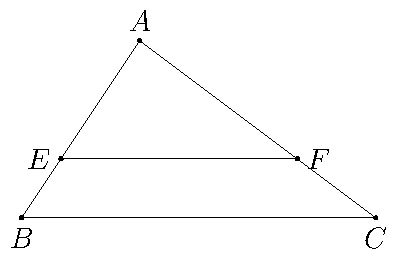
\includegraphics{analytic_geometry/thales1.pdf}
	\caption{Định lý Thales trên mặt phẳng}
	\label{thales1}
\end{figure}

Theo định lý Thales, nếu $EF$ song song với $BC$ thì ta có $\dfrac{AE}{AB} = \dfrac{AF}{AC} = \dfrac{EF}{BC}$ (hình \ref{thales1}).

Không dừng lại ở mặt phẳng, khi mở rộng lên không gian định lý Thales cũng cho chúng ta một kết quả quan trọng khi nói tới các mặt phẳng song song nhau.

\begin{theorem}[Định lý Thales trong không gian]
    Trong khối chóp, mặt phẳng song song mặt đáy chắn các cạnh nối từ đỉnh hình chóp tới các đỉnh của mặt phẳng đáy các đoạn thẳng tương ứng tỉ lệ.
\end{theorem}

\begin{figure}[ht]
	\centering
	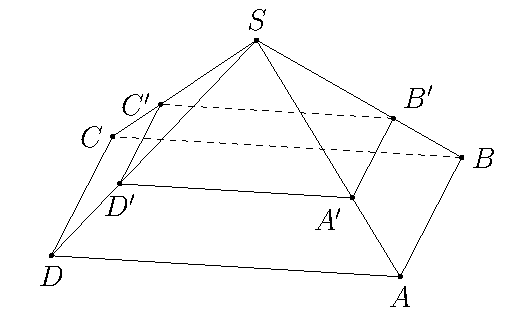
\includegraphics{analytic_geometry/thales2.pdf}
	\caption{Định lý Thales trong không gian}
	\label{thales2}
\end{figure}

Theo định lý Thales, nếu mặt phẳng $(ABCD)$ song song với mặt phẳng $(A'B'C'D')$ thì $\dfrac{SA}{SA'} = \dfrac{SB}{SB'} = \dfrac{SC}{SC'} = \dfrac{SD}{SD'}$ (hình \ref{thales2}).

\subsection*{Pythagoras của Samos}

Khi nhắc tới vuông góc, chúng ta thường nhớ tới định lý ngày nào được học ở thời học sinh: định lý Pythagoras. Định lý này nói về quan hệ giữa độ dài các cạnh trong một tam giác vuông. Định lý tuy đơn giản nhưng có ý nghĩa rất quan trọng trong đời sống và khoa học của con người suốt chiều dài lịch sử. Đây cũng là tiền đề cho định lý mang tính lịch sử của nhân loại: định lý cuối cùng của Fermat.

\begin{figure}[ht]
	\centering
	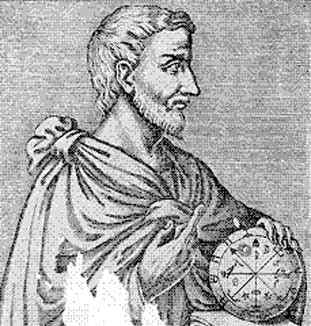
\includegraphics[scale=0.5]{analytic_geometry/Pythagoras.jpeg}
	\captionsetup{labelformat=empty}
	\caption{Pythagoras của Samos}
\end{figure}

Pythagoras của Samos cũng là nhà triết học Hy Lạp cổ, được cho rằng sinh vào khoảng năm 570 TCN và mất năm  490 TCN\footnote{\url{https://mathshistory.st-andrews.ac.uk/Biographies/Pythagoras/}}. Ông được học tập từ nhà triết học Thales và cũng có nhiều đóng góp cho sự phát triển của toán học, thiên văn học và âm nhạc. Tuy nhiên khác với thầy mình, trường phái triết học của ông cho rằng những con số là nguồn gốc của vạn vật và sử dụng những con số để giải thích những hiện tượng khoa học. Từ đây, các lý thuyết về âm nhạc được ra đời, cụ thể là các mối liên hệ về tần số với sự rung của dây nhạc cụ.

Ông là một trong những người hiếm hoi cho phép cả phụ nữ đi học ở lớp của mình vào thời ấy. Điều đó giúp phổ biến toán học nói riêng và kiến thức nói chung tới nhiều tầng lớp nhân dân. Tuy nhiên ông cũng có một hội kín rất thú vị. Như đã nói ở trên, trường phái triết học Pythagoras cố gắng giải thích nguồn gốc vạn vật bằng những con số. Điều này đã dẫn họ tới những khám phá động trời vào thời ấy.

Một trong những khám phá đó là về sự tồn tại của số vô tỉ dựa vào định lý mang tên ông. Lịch sử đã chỉ ra rằng trước Pythagoras, người Babylon và Ai Cập đã tìm ra rất nhiều bộ số nguyên $(a, b, c)$ thỏa mãn $a^2 + b^2 = c^2$ là độ dài ba cạnh tam giác vuông. Định lý Pythagoras mà ngày nay chúng ta biết được phát biểu rằng:

\begin{theorem}[Định lý Pythagoras]
    Trong một tam giác vuông, bình phương độ dài cạnh huyền bằng tổng bình phương độ dài hai cạnh góc vuông.
\end{theorem}

Như vậy nếu gọi độ dài cạnh huyền là $c$, độ dài hai cạnh góc vuông lần lượt là $a$ và $b$ thì $a^2 + b^2 = c^2$ (hình \ref{pythagoras1}).

\begin{figure}[ht]
	\centering
	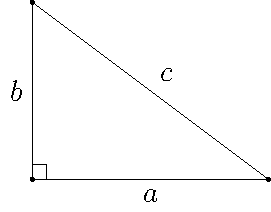
\includegraphics{analytic_geometry/pythagoras1.pdf}
	\caption{Định lý Pythagoras}
	\label{pythagoras1}
\end{figure}

Nếu $a = b = 1$ thì sao? Khi đó bình phương độ dài cạnh huyền $c^2 = 2$. Tuy nhiên không thể tìm ra một số hữu tỉ nào để bình phương lên là 2 cả. Phát hiện này là một chấn động đối với thời Pythagoras và ông yêu cầu tất cả thành viên trong hội phải giữ kín bí mật về sự phát hiện này. Tuy nhiên thông tin vẫn lọt ra ngoài và truyền thuyết kể rằng ông đã xử tội chết cho thành viên của hội không tuân thủ.

Pythagoras đã đưa một khái niệm cực kì quan trọng trong toán học, gọi là \textit{chứng minh} (proof). Để chứng minh một mệnh đề là đúng, chúng ta cần các mệnh đề (thường đơn giản hơn) đúng trước đó. Bằng các phép suy luận thích hợp dựa trên các mệnh đề đúng trước đó, chúng ta có thể kết luận rằng mệnh đề cần chứng minh là đúng. Phép chứng minh có thể gọi là \textit{xương sống} của toán học, vì nếu không có một phép chứng minh đúng đắn thì một mệnh đề không thể được xác định được là có đúng hay không. Trong trường hợp của Fermat, khi ông đưa ra định lý Fermat nhưng không kèm chứng minh (vì lề sách quá chật nên không viết lời giải được) thì chúng ta không thể biết định lý Fermat có đúng hay không (?).

Nếu việc suy luận dựa trên các mệnh đề, hoặc định lý, đã đúng trước đó, thì phải có một lúc nào đó việc này dừng lại. Chúng ta không thể suy ngược tới vô hạn lần được. Do đó chúng ta cần những mệnh đề luôn đúng nhưng tính đúng đắn của nó được kiểm nghiệm trong thực tiễn. Chúng được gọi là \textit{tiên đề} (axiom). Nhân vật tiếp theo được đề cập tới sẽ dẫn chúng ta tới hệ thống tiên đề làm nền tảng cho hình học.

\subsection*{Euclid của Alexandria}

Đúng vậy, Euclid là người đặt nền móng cho hình học với bộ sách nổi tiếng \textit{Elements} của mình. Trong bộ sách này đề cập tới những tiên đề, định lý làm nền tảng cho bộ môn hình học và vẫn còn ý nghĩa cho tới tận ngày nay. Những gì viết trong đó không quá xa lạ với những gì được giảng dạy trong nhà trường.

\begin{figure}[ht]
	\centering
	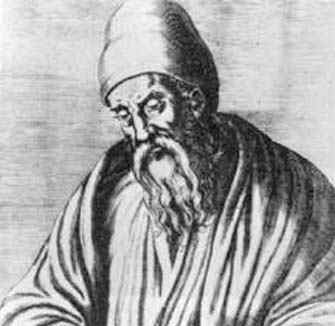
\includegraphics[scale=0.5]{analytic_geometry/Euclid.jpeg}
	\captionsetup{labelformat=empty}
	\caption{Euclid của Alexandria}
\end{figure}

Euclid của Alexandria sinh vào khoảng năm 325 TCN và mất vào khoảng năm 265 TCN\footnote{\url{https://mathshistory.st-andrews.ac.uk/Biographies/Euclid/}}. Thông tin về ông không có nhiều. Nhưng chỉ mỗi bộ sách \textit{Elements} cũng đủ để người đời sau cho rằng ông là người có ảnh hưởng nhất trong 2000 năm lịch sử phát triển của toán học.

Năm tiên đề cơ bản của hình học được ông phát biểu trong bộ \textit{Elements} được phát biểu như sau:

\begin{enumerate}
	\item Qua hai điểm bất kì luôn vẽ được một đường thẳng
	\item Đường thẳng có thể kéo dài vô hạn về cả hai phía
	\item Ta có thể xác định một đường tròn bằng tâm và bán kính của nó
	\item Mọi góc vuông đều bằng nhau
	\item Nếu một đường thẳng cắt hai đường thẳng khiến tổng hai góc trong cùng phía nhỏ hơn hai vuông thì hai đường thẳng đó chắc chắn sẽ cắt nhau tại một điểm nào đó
\end{enumerate}

Tiên đề số 5 là rắc rối và phức tạp nhất. Nó không thực sự tự nhiên và có nhiều sự vướng mắc. Đây chính là tiên đề cho sự ra đời của hình học phi-Euclid hơn 1500 năm sau.

Bộ \textit{Elements} của Euclid bao gồm 13 quyển. Trong đó đề cập tới rất nhiều vấn đề của hình học, từ những phần tử đơn giản nhất cấu tạo nên hình học là điểm, đoạn thẳng, đường thẳng, tới những hình học lớn hơn như hình chữ nhật, hình tròn, đa giác, mặt phẳng. Thậm chí ông cũng đã có những dấu chân ở hình học không gian như hình chóp, hình cầu, hình nón (\cite{Euclid}, \cite{Casey2007}).

\section{Phương pháp tọa độ trong mặt phẳng}

Cuộc cách mạng trong hình học xảy ra khi nhà toán học lãng tử René Descartes phát minh ra hệ tọa độ và từ đó mọi đối tượng hình học có thể được biểu diễn bởi các phương pháp đại số như phương trình, đẳng thức.

\begin{figure}[ht]
	\centering
	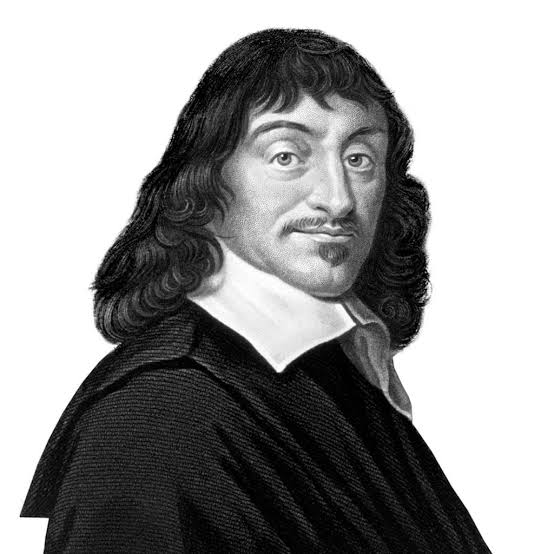
\includegraphics[scale=0.5]{mathematicians/Descartes.jpg}
	\captionsetup{labelformat=empty}
	\caption{René Descartes (1596-1650)}
\end{figure}

\subsection*{Danh mục thuật ngữ và ký hiệu}

Đầu tiên chúng ta thống nhất các thuật ngữ cũng như ký hiệu được sử dụng kể từ đây.

\textbf{Điểm} là đơn vị cơ bản của hình học. Bất kì đối tượng hình học nào cũng là một \textit{tập hợp điểm}. Điểm được ký hiệu bởi chữ in hoa, ví dụ như $A$, $B_1$, $B_2$.

\textbf{Đường thẳng} đi qua hai điểm phân biệt cho trước. Đường thẳng có thể kéo dài vô hạn về hai phía. Đường thẳng được ký hiệu bởi chữ in thường hoặc chữ Hy Lạp trong ngoặc đơn, ví dụ như $(d)$, $(\Delta)$.

\textbf{Đoạn thẳng} chỉ phần đường thẳng nằm giữa hai điểm.

\textbf{Nửa đường thẳng} chỉ phần đường thẳng nằm một phía của một điểm trên đường thẳng và chỉ kéo dài vô hạn về phía đó.

\textbf{Vector} là đoạn thẳng có hướng. Với điểm đầu là $A$ và điểm cuối là $B$ thì vector từ $A$ tới $B$ được ký hiệu là $\overrightarrow{AB}$. Để chỉ một vector không cần biết điểm đầu và điểm cuối ta dùng chữ thường in đậm, ví dụ như $\bm{a}$.

\textbf{Góc giữa hai vector} $\overrightarrow{OA}$ và $\overrightarrow{OB}$ là góc $\angle AOB$ và ký hiệu là $(\overrightarrow{OA}, \overrightarrow{OB})$.

Tương tự đối với vector $\bm{a}$ và $\bm{b}$ thì góc giữa chúng ký hiệu là $(\bm{a}, \bm{b})$.

\subsection*{Vector trong mặt phẳng}

Trong hệ tọa độ $Oxy$ với tâm $O$ và hai trục $Ox$ (trục hoành) và $Oy$ (trục tung) vuông góc nhau, đặt $O = (0, 0)$ là tọa độ của tâm $O$.

Tiếp theo, mọi điểm trong mặt phẳng Euclid đi liền với cặp số $(x, y)$ chỉ tọa độ của điểm đó. Ví dụ $A = (1, 3)$, $B = (4, 1)$.

\begin{figure}[ht]
	\centering
	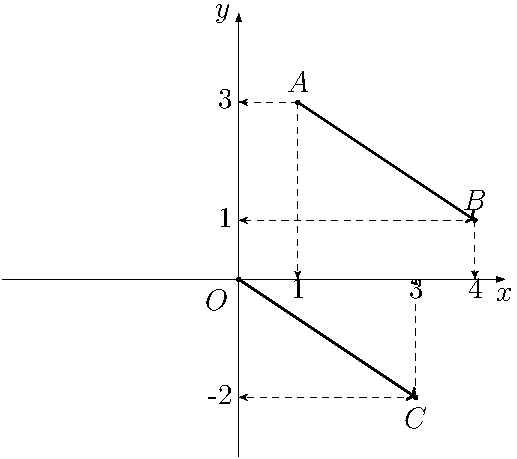
\includegraphics[page=1]{analytic_geometry/oxy1.pdf}
	\caption{Tọa độ của điểm trong mặt phẳng}
	\label{oxy1}
\end{figure}

Tọa độ của điểm cũng là tọa độ của vector từ $O$ tới điểm đó. Với hình \ref{oxy1} thì $\overrightarrow{OA} = (1, 3)$ và $\overrightarrow{OB} = (4, 1)$. Tọa độ của vector $\overrightarrow{AB}$ khi đó sẽ là $\overrightarrow{AB} = \overrightarrow{OB} - \overrightarrow{OA} = (4, 1) - (1, 3) = (3, -2)$. Cũng theo hình \ref{oxy1} thì ta thấy $\overrightarrow{AB} = \overrightarrow{OC} = (3, -2)$. 

Như vậy, nếu ta có hai điểm $A = (x_A, y_A)$ và $B = (x_B, y_B)$ thì vector $\overrightarrow{AB}$ là
\begin{equation}
	\overrightarrow{AB} = (x_B - x_A, y_B - y_A)
\end{equation}

\textbf{Tích vô hướng của hai vector} $\bm{a} = (x_1, y_1)$ và $\bm{b} = (x_2, y_2)$ được định nghĩa là
\begin{equation}
	\langle \bm{a}, \bm{b} \rangle = x_1 x_2 + y_1 y_2
\end{equation}

Ta cũng có thể ký hiệu tích vô hướng là $\bm{a} \cdot \bm{b}$.

Ta ký hiệu $\lVert \bm{a} \rVert$ là độ dài (chuẩn Euclid, Euclid norm) của vector $\bm{a}$. Trong hệ tọa độ Descartes vuông góc, theo định lý Pythagoras, độ dài của vector là độ dài cạnh huyền tam giác vuông (hình \ref{oxy1}). Như vậy, độ dài đoạn thẳng $AB$ với $A = (x_A, y_A)$ và $B = (x_B, y_B)$ là
\begin{equation}
	AB = \lVert \overrightarrow{AB} \rVert = \sqrt{(x_B - x_A)^2 + (y_B - y_A)^2}
\end{equation}

Khi đó cosin góc giữa hai vector $\bm{a}$ và $\bm{b}$ là
\begin{equation}
	\cos (\bm{a}, \bm{b}) = \frac{\bm{a} \cdot \bm{b}}{\lVert \bm{a} \rVert \cdot \lVert \bm{b} \rVert} = \frac{x_1 x_2 + y_1 y_2}{\sqrt{x_1^2 + y_1^2} \cdot \sqrt{x_2^2 + y_2^2}}
\end{equation}

Nếu góc giữa hai vector bằng 90 độ thì hai vector được gọi là vuông góc nhau. Khi đó tích vô hướng $\bm{a} \cdot \bm{b} = 0$.

\subsection*{Phương trình đường thẳng trong mặt phẳng}

Theo tiên đề Euclid, một đường thẳng được xác định khi biết hai điểm phân biệt thuộc đường thẳng đó. Trong hệ tọa độ, chúng ta có hai cách tìm phương trình đường thẳng.

\textbf{Bằng vector pháp tuyến}. Vector pháp tuyến của đường thẳng là vector vuông góc với mọi vector có phương là đường thẳng đó. Giả sử $\bm{v} = (a, b)$ là vector pháp tuyến của đường thẳng đi qua điểm $M_0 = (x_0, y_0)$. Khi đó đường thẳng đi qua qua $M_0$ nhận $\bm{v}$ làm vector pháp tuyến là \textit{tập hợp điểm} $M = (x, y)$ trên mặt phẳng sao cho $\bm{v} \cdot \overrightarrow{M_0 M} = 0$. Điều này tương đương với
\begin{equation}
	\bm{v} \cdot \overrightarrow{M_0 M} = a \cdot (x - x_0) + b \cdot (y - y_0) = 0
\end{equation}

\textbf{Bằng vector chỉ phương}. Vector chỉ phương của đường thẳng là vector có phương song song với đường thẳng đó. Giả sử $\bm{v}' = (a', b')$ là vector chỉ phương của đường thẳng đi qua điểm $M_0 = (x_0, y_0)$. Khi đó đường thẳng đi qua $M_0$ nhận $\bm{v}'$ làm vector chỉ phương là \textit{tập hợp điểm} $M = (x, y)$ trên mặt phẳng sao cho $\bm{v}' \parallel \overrightarrow{M_0 M}$. Điều này tương đương với
\begin{equation}
	\bm{v}' \parallel \overrightarrow{M_0 M} \Leftrightarrow \frac{x - x_0}{a'} = \frac{y - y_0}{b'}
\end{equation}

\begin{enumerate}
	\item Cả hai cách biểu diễn khi khai triển ra đều có dạng $a x + by + c = 0$ với $c$ là hằng số. Đây được gọi là dạng tổng quát của phương trình đường thẳng. 
	
	\item Cách viết $\dfrac{x - x_0}{a'} = \dfrac{y - y_0}{b'}$ được gọi là dạng chính tắc của phương trình đường thẳng.
	
	\item Dạng chính tắc của phương trình đường thẳng còn có một tác dụng đặc biệt khác \[\frac{x - x_0}{a'} = \frac{y - y_0}{b'} = t\] với $t \in \mathbb{R}$. Khi đó tọa độ $M = (x, y)$ có thể được biểu diễn dưới dạng
	\begin{equation}
		\begin{cases}
			x = x_0 + a' t \\ y = y_0 + b' t
		\end{cases}, \quad t \in \mathbb{R}
	\end{equation}
	Đây được gọi là phương trình dạng tham số.
\end{enumerate}

Chúng ta chú ý rằng nếu đường thẳng song song với một trong hai trục tọa độ thì vector chỉ phương của nó sẽ cùng phương với vector đơn vị $(1, 0)$ hoặc $(0, 1)$. Do đó không thể viết dưới dạng chính tắc được (không thể chia cho 0) nhưng có thể viết dưới dạng tổng quát hoặc dạng tham số.

\subsection*{Khoảng cách giữa điểm và đường thẳng}

Nhắc lại một chút kiến thức cơ sở. \textbf{Khoảng cách} từ một điểm $A$ nằm ngoài đường thẳng $(d)$ là độ dài đoạn thẳng $AH$ với $H \in (d)$ sao cho $AH$ nhỏ nhất (hình \ref{oxy2}).

Khi đó $H$ được gọi là \textbf{hình chiếu} của $A$ lên đường thẳng $(d)$ và $AH$ là \textbf{khoảng cách} từ $A$ tới $(d)$. Do $AH$ là đoạn thẳng có độ dài ngắn nhất, điều này xảy ra khi $AH \perp (d)$.

\begin{figure}[ht]
	\centering
	\includegraphics[page=2]{analytic_geometry/oxy1.pdf}
	\caption{Hình chiếu và khoảng cách tới đường thẳng}
	\label{oxy2}
\end{figure}

Như vậy, để tìm hình chiếu của điểm $A$ lên đường thẳng $(d)$, ta dựng đường thẳng đi qua điểm $A$ và vuông góc với $(d)$.

Giả sử phương trình đường thẳng $(d)$ với vector pháp tuyến $\bm{v} = (a, b)$ là $(d): ax + by + c = 0$.

Gọi $(d')$ là đường thẳng đi qua $A = (x_0, y_0)$ và vuông góc với $d$. Do $\bm{v}$ là vector pháp tuyến của $(d)$ nên $\bm{v}$ là vector chỉ phương của $(d')$. Khi đó phương trình dạng tham số của $(d')$ là \[\begin{cases}
	x = x_0 + a t \\ y = y_0 + b t
\end{cases}, t \in \mathbb{R}\]

Gọi $H$ là hình chiếu của $A$ lên $(d)$. Khi đó $H$ là giao điểm của $(d)$ và $(d')$. Vì $H \in (d')$ nên tọa độ của $H$ có dạng $(x_0 + at, y_0 + bt)$ với $t$ nào đó thuộc $\mathbb{R}$. Chúng ta sẽ đi tìm $t$ này.

Vì $H \in (d)$ nên ta thay tọa độ của $H$ vừa tìm được vào phương trình của $(d)$ thu được \[a (x_0 + at) + b (y_0 + bt) + c = 0 \Leftrightarrow t = -\frac{a x_0 + b y_0 + c}{a^2 + b^2}\]
Như vậy là ta đã tìm được $t$ từ đó xác định được tọa độ của $H$.

Từ đây ta tính được khoảng cách từ $A$ tới $(d)$ hay nói cách khác là độ dài đường $AH$. Ta có $A = (x_0, y_0)$ và $H = (x_0 + at, y_0 + bt)$ nên $\overrightarrow{AH} = (at, bt)$. Suy ra
\begin{align*}
	AH = & \lVert \overrightarrow{AH} \rVert = \sqrt{(at)^2 + (bt)^2} = \lvert t \rvert \sqrt{a^2 + b^2} \\ = & \Big| -\frac{a x_0 + b y_0 + c}{a^2 + b^2} \Big| \cdot \sqrt{a^2 + b^2} = \frac{\lvert a x_0 + b y_0 + c \rvert}{\sqrt{a^2 + b^2}}
\end{align*}

\section{Đạo hàm}

Phép tính vi tích phân đã được con người nghiên cứu từ lâu. Câu chuyện về ai là người phát minh ra phép tính vi tích phân: Newton hay Leibniz, được coi là một trong những vụ tranh cãi đáng xấu hổ nhất lịch sử toán học. Nhưng họ cũng đã để lại một mảnh đất màu mỡ cho toán học về sau.

\subsection*{Cơ học và sự ra đời của đạo hàm}

Trường phái Newton sử dụng đạo hàm như công cụ khảo sát vận tốc từ quãng đường. Ở bậc trung học chúng ta biết rằng \textit{vận tốc trung bình} bằng quãng đường chia thời gian. Tuy nhiên điều đó chỉ đúng cho \textit{chuyển động thẳng đều}. Nếu quãng đường là một hàm số phụ thuộc thời gian (quãng đường là $s(t)$ với $t$ là thời gian) thì điều đó không đúng nữa.

Do quãng đường phụ thuộc thời gian nên có thể là vận tốc cũng phụ thuộc thời gian? Hợp lí đấy. Nhưng với mỗi một giá trị thời gian $t$ cho ta một vị trí $s(t)$ trên trục số, còn vận tốc thì không thể phụ thuộc một giá trị thời gian được. Rõ ràng vật phải di chuyển một quãng đường từ thời gian $t_0$ tới $t_1$ thì mới có vận tốc trên quãng đường đó chứ?

Cách tiếp cận ở đây là, chúng ta cho sự thay đổi thời gian, tức hiệu $\Delta t = t_1 - t_0$, rất nhỏ. Khi đó vật đi từ $s(t_0)$ tới $s(t_1)$, vậy là chúng ta có thể tính vận tốc với công thức $v = \dfrac{s(t_1) - s(t_0)}{t_1 - t_0}$. Do $\Delta t$ rất nhỏ, hay \textit{tiến về 0}, thì vận tốc gần như xảy ra vào đúng một thời điểm. Do đó vận tốc lúc này được gọi là \textit{vận tốc tức thời}. Đó cũng chính là ý nghĩa cơ học và sự ra đời của đạo hàm theo trường phái Newton.

\subsection*{Định nghĩa đạo hàm}

Xét hàm số $f(x)$ liên tục trên khoảng $(a, b)$ có chứa điểm $x_0$. Đạo hàm của $f(x)$ tại $x_0$ được định nghĩa là giới hạn
\begin{equation}
	f'(x_0) = \lim_{x \to x_0} \frac{f(x) - f(x_0)}{x - x_0}
	\label{der1}
\end{equation}

Lưu ý rằng nếu giới hạn trên không phải là giới hạn hữu hạn (không tồn tại hoặc tiến tới vô cực) thì hàm số không có đạo hàm tại điểm $x_0$.

Ví dụ, để tính đạo hàm của hàm số $f(x) = x^3 + 2 x^2 - 4$ tại $x_0 = 4$, ta khai triển
\begin{align*}
	\frac{f(x) - f(x_0)}{x - x_0} = & \frac{f(x) - f(4)}{x - 4} \\ = & \frac{x^3 + 2x^2 - 4 - (4^3 + 2 \cdot 4^2 - 4)}{x - 4} \\ = & \frac{(x^3 - 4^3) + 2(x^2 - 4^2)}{x - 4} \\ = & \frac{(x-4)(x^2 + 4x + 16) + 2 (x-4)(x+4)}{x - 4} \\ = & x^2 + 4 x + 16 + 2(x+4)
\end{align*}

Cho $x$ tiến tới 4 thì ta có đạo hàm tại $x = 4$
\begin{align*}
	f'(4) = & \lim_{x \to 4} \frac{f(x) - f(4)}{x - 4} \\ = & \lim_{x \to 4} (x^2 + 4x + 16 + 2(x+4)) \\ = & 4^2 + 4 \cdot 4 + 16 + 2 \cdot (4 + 4) = 64
\end{align*}

Trong định nghĩa ở \ref{der1}, nếu ta đặt $\Delta x = x - x_0$ và $\Delta y = y - y_0 = f(x) - f(x_0)$, ta gọi $\Delta x$ là \textit{số gia} của biến $x$, tương tự $\Delta y$ là \textit{số gia} của biến $y$.

Trong định nghĩa, $x$ tiến tới $x_0$ tương đương với $\Delta x$ tiến tới 0. Chuyển vế $x_0$ ta có $x = x_0 + \Delta x$ và từ đó $f(x) = f(x_0 + \Delta x)$. Định nghĩa đạo hàm ở trên có thể được viết lại
\begin{equation}
	f'(x_0) = \lim_{\Delta x \to 0} \frac{f(x_0 + \Delta x) - f(x_0)}{\Delta x} = \lim_{\Delta x \to 0} \frac{\Delta y}{\Delta x}
\end{equation}

Nếu hàm số có đạo hàm tại mọi điểm trên khoảng $(a, b)$ thì ta nói hàm số khả vi trên khoảng đó.

Ví dụ đối với hàm số $f(x) = x^3 + 2x^2 - 4$ như trên. Với mọi $x_0 \in \mathbb{R}$ ta có
\begin{align*}
	f'(x_0) = & \lim_{x \to x_0} \frac{f(x) - f(x_0)}{x - x_0} \\ = & \lim_{x \to x_0} \frac{x^3 + 2x^2 - 4 - (x_0^3 + 2x_0^2 - 4)}{x - x_0} \\ = & \lim_{x \to x_0} \frac{(x^3 - x_0^3) + 2 (x^2 - x_0^2)}{x - x_0} \\ = & \lim_{x \to x_0} (x^2 + x x_0 + x_0^2) + 2 (x + x_0) \\ = & x_0^2 + x_0 \cdot x_0 + x_0^2 + 2 (x_0 + x_0) = 3x_0^2 + 4 x_0
\end{align*}

Ta thấy rằng giới hạn trên luôn tồn tại với mọi $x_0 \in \mathbb{R}$ nên thay $x_0$ thành $x$ ta có đạo hàm $f'(x) = 3x^2 + 4x$ của $f(x)$ trên $\mathbb{R}$.

\subsection*{Vi phân}

Trong cách ký hiệu \[f'(x) = \lim_{\Delta x \to 0} \frac{\Delta y}{\Delta x}\] ta thay $\Delta y$ thành $dy$ và $\Delta x$ thành $dx$ thì vi phân được định nghĩa là 
\begin{equation}
	f'(x) = \frac{dy}{dx} \Leftrightarrow dy = f'(x)\, dx
\end{equation}

Cách ký hiệu vi phân có ý nghĩa là vế trái là vi phân theo biến $y$ và vế phải là vi phân theo biến $x$. Do $y = f(x)$ nên khi vi phân hai vế sẽ cho ra $dy = f'(x)\, dx$ (vế trái là đa thức bậc 1 biến $y$).

Ví dụ phương trình $y^2 = x^3 + 4x - 7$ thì khi vi phân hai vế ta có \[(y^2)' \, dy = (x^3 + 4x - 7) \, dx \Leftrightarrow 2y \, dy = (3x^2 + 4) \, dx\]

\subsection*{Ý nghĩa hình học của đạo hàm}

Xét hàm số $y = f(x)$ liên tục trên khoảng $(a, b)$ chứa điểm $x_0$.

Gọi $M' = (x, y)$ là một điểm thuộc hàm số $y = f(x)$. Khi đó đạo hàm của $f(x)$ tại $x_0$ là giới hạn  \[\lim_{x \to x_0} \frac{f(x) - f(x_0)}{x - x_0} = \lim_{\Delta x \to 0} \frac{f(x_0 + \Delta x) - f(x_0)}{\Delta x} = \lim_{\Delta x \to 0} \frac{\Delta y}{\Delta x}\]

Xét hình \ref{int2a}, tỉ số $\Delta y / \Delta x$ là tangent của góc hợp bởi trục hoành $Ox$ và đường thẳng $MM'$.

\begin{figure}[ht]
	\centering
	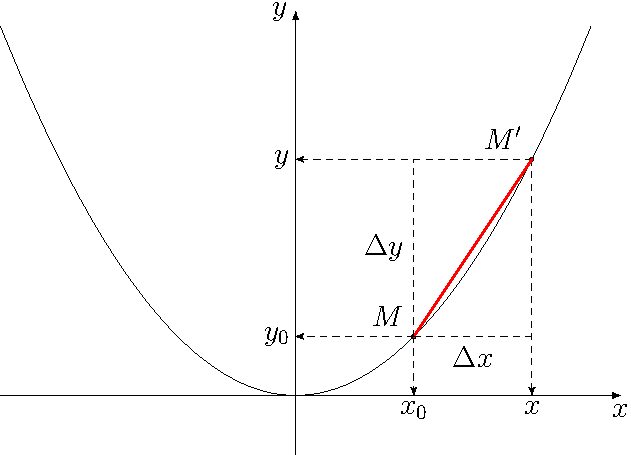
\includegraphics[page=1,scale=0.75]{analytic_geometry/int2.pdf}
	\caption{Hệ số góc (trường hợp 1)}
	\label{int2a}
\end{figure}

Tiếp theo, xét hình \ref{int2b}, ta thấy đường thẳng $MM'$ ngày càng tiến sát lại với đường cong. Như vậy, khi $\Delta x$ tiến tới 0 thì đường thẳng $MM'$ cắt đường cong tại hai điểm càng sát nhau. Đến khi hai điểm đó trùng nhau, đường thẳng $MM'$ chỉ đi qua đúng một điểm thuộc đường cong và khi đó $MM'$ trở thành tiếp tuyến của đường cong tại điểm $M = (x_0, y_0)$.

\begin{figure}[ht]
	\centering
	\includegraphics[page=2,scale=0.75]{analytic_geometry/int2.pdf}
	\caption{Hệ số góc (trường hợp 2)}
	\label{int2b}
\end{figure}

Khi đó $f'(x_0)$ là tangent của góc hợp bởi $MM'$ và trục hoành $Ox$, hay nói cách khác là \textit{hệ số góc} của đường tiếp tuyến. Thêm nữa $f'(x_0) = \dfrac{\Delta y}{\Delta x} = \dfrac{y - y_0}{x - x_0}$ nên phương trình đường tiếp tuyến đi qua $M = (x_0, y_0)$ là
\begin{equation}
	y = f'(x_0) (x - x_0) + y_0
\end{equation}

\section{Tích phân}

Tích phân là khái niệm quan trọng trong giải tích. Sau đây sẽ trình bày cách tính tích phân theo tổng Riemann.

\subsection*{Tích phân và phân chia diện tích}

Xét phương trình của một đường cong $y = f(x) > 0$ trên đoạn $[a, b]$.

Theo định nghĩa, tích phân từ $a$ tới $b$ là diện tích phần hình phẳng giới hạn bởi đường cong $y = f(x)$, trục hoành $Ox$ và hai trục đứng $x = a$, $x = b$.

Ờ hình \ref{int1}, diện tích phần tô màu xám là tích phân từ -2 tới 2 của hàm số $f(x) = -x^2 + 4$.

\begin{figure}[ht]
	\centering
	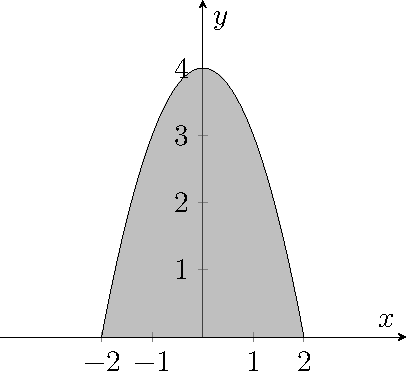
\includegraphics[page=1]{analytic_geometry/int1.pdf}
	\caption{Tích phân từ -2 tới 2 của $f(x) = -x^2 + 4$}
	\label{int1}
\end{figure}

Chúng ta có thể tính diện tích hình chữ nhật, hình thang, hình vuông. Vậy có cách nào để tính diện tích một hình giới hạn bởi các đường cong bất kì không? Có đấy. Chúng ta sẽ tính xấp xỉ bằng tổng diện tích các hình chữ nhật.

Ví dụ với hàm số $f(x) = -x^2 + 4$ ở trên, ta chia đoạn $[a, b]$ thành $n$ phần bằng nhau \[a = x_0 < x_1 < \ldots < x_{n-1} < x_n = b\]
Trong đó $x_{i+1} - x_i$ cố định và bằng $\dfrac{b-a}{n}$.

Đối với hình \ref{int2} ta xấp xỉ bằng 7 hình chữ nhật. Đối với hình \ref{int3} ta xấp xỉ bằng 15 hình chữ nhật. Đối với hình \ref{int4} ta xấp xỉ bằng 31 hình chữ nhật. 

\begin{figure}[htb]
	\centering
	\includegraphics[page=2]{analytic_geometry/int1.pdf}
	\caption{Xấp xỉ diện tích bởi 7 hình chữ nhật}
	\label{int2}
\end{figure}

\begin{figure}[htb]
	\centering
	\includegraphics[page=3]{analytic_geometry/int1.pdf}
	\caption{Xấp xỉ diện tích bởi 15 hình chữ nhật}
	\label{int3}
\end{figure}

\begin{figure}[htb]
	\centering
	\includegraphics[page=4]{analytic_geometry/int1.pdf}
	\caption{Xấp xỉ diện tích bởi 31 hình chữ nhật}
	\label{int4}
\end{figure}

Càng dùng nhiều hình chữ nhật, tổng diện tích của chúng càng gần với diện tích cần tìm, hay là tích phân cần tìm.

Ở ba hình trên, mỗi hình chữ nhật trong đó có chiều rộng bằng nhau là $\dfrac{b-a}{n}$ với $n$ là số đoạn. Chiều dài là $f(x_i)$ với $x_i = a + \dfrac{b-a}{n} i$, $i = 1, 2, \ldots, n$ (biên sau).

Cụ thể hơn, hình chữ nhật từ $x_{i-1}$ tới $x_i$ sẽ có chiều dài là $f(x_i)$ và chiều rộng là $\dfrac{b-a}{n}$. % Việc chọn chiều dài không bắt buộc phải chọn biên sau. Chúng ta hoàn toàn có thể chọn chiều dài là $f(x_{i-1})$, hoặc $\max f(x)$, $\min f(x)$ trên đoạn $[x_{i-1}, x_i]$.

Khi đó, tổng diện tích của các hình chữ nhật là
\begin{equation}
	\sum_{i=1}^n (x_{i} - x_{i-1}) f(x_i) = \sum_{i=1}^n \frac{b-a}{n} f(x_i)
\end{equation}

Khi số lượng hình chữ nhật tăng lên tới vô hạn thì tổng diện tích sẽ tiến tới diện tích chính xác của hình cần tìm, hay nói cách khác là tích phân. Do đó kết quả sẽ là
\begin{equation}
	\int\displaylimits_{a}^{b} f(x)\,dx = \lim_{n \to \infty} \sum_{i=1}^{n} \frac{b-a}{n} f(x_i), \quad x_i = a + \frac{b-a}{n} i
\end{equation}

\subsection*{Ví dụ tính tích phân qua tổng Riemann}

Ví dụ, tính tích phân từ -2 tới 2 của hàm số $f(x) = -x^2 + 4$ ở trên. Ta có $b = 2$ và $a = -2$ nên \begin{align*}
	\frac{b-a}{n} f(x_i) = & \frac{4}{n} \Bigl(-\Bigl(-2+\frac{4}{n} i\Bigr)^2 + 4\Bigr) \\ = & \frac{4}{n}\Bigl( -4 + \frac{16}{n} i - \frac{16}{n^2} i^2 + 4\Bigr) \\ = & \frac{64}{n} \Bigl( \frac{i}{n} - \frac{i^2}{n^2} \Bigr)
\end{align*}

Tính tổng $i$ từ 1 tới $n$ ta có $\displaystyle{\sum_{i=1}^{n} i = \frac{n(n+1)}{2}}$.

Tính tổng $i^2$ từ 1 tới $n$ ta có $\displaystyle{\sum_{i=1}^{n} i^2 = \frac{n(n+1)(2n+1)}{6}}$.

Suy ra
\begin{align*}
	\sum_{i=1}^n \frac{64}{n} \Bigl(\frac{i}{n} - \frac{i^2}{n^2}\Bigr) = & \frac{64}{n^2} \sum_{i=1}^n i - \frac{64}{n^3} \sum_{i=1}^{n} i^2 \\ & = -\frac{64}{n^2} \cdot \frac{n(n+1)}{2} - \frac{64}{n^3} \cdot \frac{n(n+1)(2n+1)}{6}
\end{align*}

Khi $n$ tiến tới vô cực thì biểu thức trên tiến tới $\dfrac{64}{2} - \dfrac{64 \cdot 2}{6} = \dfrac{32}{3}$. Đây chính là giá trị của tích phân $\displaystyle{\int\displaylimits_{-2}^2 (-x^2 + 4) \, dx}$.

\chapter{Machine Learning}

\section{Linear Regression}

Giả sử ta có $N$ điểm dữ liệu đầu vào $\bm{x}_1, \bm{x}_2, \ldots, \bm{x}_N$ với $\bm{x}_i \in \RR^d$. Ứng với từng điểm dữ liệu đầu vào $\bm{x}_i$ ta có một đầu ra $y_i$. Nghĩa là ta có $N$ cặp dữ liệu $(\bm{x}_i, y_i)$.

Mục tiêu là xây dựng hàm số $\hat{y} = f(x_1, x_2, \ldots, x_d)$ sao cho tổng sai số của $y_i$ và $\hat{y}_i$ là nhỏ nhất, tức là \[ \sum_{i=1}^N \lVert y_i - \hat{y}_i \rVert^2 \to \min \]

Để hàm số đạt giá trị nhỏ nhất (hoặc lớn nhất) ta tìm cực trị của hàm số và khảo sát. Tuy nhiên không phải hàm số nào cũng đạo hàm được. Một cách tiếp cận đơn giản là sử dụng hàm tuyến tính, dễ xây dựng và luôn khả vi. Ta đặt \[ \hat{y} = f(x_1, x_2, \ldots, x_d) = w_0 + w_1 x_1 + w_2 x_2 + \ldots + w_d x_d \]

Lúc này, hàm mất mát ở trên có dạng \[ \mathcal{L} = \sum_{i=1}^N \lVert y_i - (w_0 + w_1 x_{i1} + w_2 x_{i2} + \ldots + w_d x_{id} \rVert^2 \]

Bình phương chuẩn Euclid chính là bình phương của vector. Do đó dưới dấu tổng là các hàm số bình phương. Khi đạo hàm riêng theo $w_j$ ta có \[ \dfrac{\partial \mathcal{L}}{\partial w_j} = \sum_{i=1}^N 2 x_{ij} (y_i - (w_0 + w_1 x_{i1} + w_2 x_{i2} + \ldots + w_d x_{id})) \] với $1 \leq j \leq d$. Với $j = 0$ có chút khác biệt, $\dfrac{\partial \mathcal{L}}{\partial w_0} = \sum_{i=1}^N 2 (y_i - (w_0 + w_1 x_{i1} + \ldots + w_d x_{id}))$.

Ta cho các đạo hàm riêng $\dfrac{\partial \mathcal{L}}{\partial w_j}$ bằng 0 thì được
\begin{align*}
    \sum_{i=1}^N x_{ij} (w_0 + w_1 x_{i1} + w_2 x_{i2} + \ldots + w_d x_{id}) & = \sum_{i=1}^N x_{ij} y_i \\ \Leftrightarrow w_0 \sum_{i=1}^N x_{ij} + w_1 \sum_{i=1}^N x_{ij} x_{i1} + w_2 \sum_{i=1}^N x_{ij} x_{i2} \\ + \cdots + w_d \sum_{i=1}^N x_{ij} x_{id} & = \sum_{i=1}^N x_{ij} y_i
\end{align*}

Bây giờ chúng ta cần biểu diễn các dấu tổng lại thành dạng đại số (ma trận, vector) vì chúng sẽ được sử dụng để nhân với vector $\bm{w} = (w_0, w_1, \ldots, w_d)$.

Ta có $\sum_{i=1}^N x_{ij} = \begin{pmatrix}
    1 & 1 & \cdots & 1
\end{pmatrix} \cdot \begin{pmatrix}
    x_{1j} \\ x_{2j} \\ \vdots \\ x_{Nj}
\end{pmatrix}$.

Ta cũng có $\sum_{i=1}^N x_{ij} x_{i1} = \begin{pmatrix}
    x_{11} & x_{21} & \cdots & x_{N1}
\end{pmatrix} \cdot \begin{pmatrix}
    x_{1j} \\ x_{2j} \\ \vdots \\ x_{Nj}
\end{pmatrix}$.

Cứ tương tự như vậy, ta xếp các dấu sigma thành dạng cột thì tương đương với \[\begin{pmatrix}
    * & \sum_{i=1}^N x_{ij} & * \\ * & \sum_{i=1}^N x_{ij} x_{i1} & * \\ \vdots & \vdots & \vdots \\ * & \sum_{i=1}^N x_{ij} x_{id} & *
\end{pmatrix} = \begin{pmatrix}
    1 & 1 & \cdots & 1 \\ x_{11} & x_{21} & \cdots & x_{N1} \\ \cdots & \cdots & \ddots & \cdots \\ x_{1d} & x_{2d} & \cdots & x_{Nd} 
\end{pmatrix} \cdot \begin{pmatrix}
    * & x_{1j} & * \\ * & x_{2j} & * \\ \vdots & \vdots & \vdots \\ * & x_{Nj} & *
\end{pmatrix}\]

Ghép các cột theo thứ tự $j$ từ 0 tới $d$ ta có
\begin{align*}
    \begin{pmatrix}
        w_0 & w_1 & \cdots & w_d
    \end{pmatrix} & \cdot \begin{pmatrix}
        1 & 1 & \cdots & 1 \\ x_{11} & x_{21} & \cdots & x_{N1} \\ \cdots & \cdots & \ddots & \cdots \\ x_{1d} & x_{2d} & \cdots & x_{Nd}
    \end{pmatrix} \\ & \times \begin{pmatrix}
        1 & x_{11} & \cdots & x_{1d} \\ 1 & x_{21} & \cdots & x_{2d} \\ \cdots & \cdots & \ddots & \cdots \\ 1 & x_{N1} & \cdots & x_{Nd}
    \end{pmatrix} \\ = \begin{pmatrix}
        y_1 & y_2 & \cdots & y_N
    \end{pmatrix} & \cdot \begin{pmatrix}
        1 & x_{11} & \cdots & x_{1d} \\ 1 & x_{21} & \cdots & x_{2d} \\ \cdots & \cdots & \ddots & \cdots \\ 1 & x_{N1} & \cdots & x_{Nd}
    \end{pmatrix}
\end{align*}

Hay nói cách khác, nếu ta đặt $\bm{w} = (w_0, w_1, \ldots, w_d)$ là ma trận hàng, $\bm{X}$ là ma trận có các hàng là các input, thì phương trình trên được viết lại là $\bm{w} \bm{X}^T \bm{X} = \bm{y} \bm{X}$.

Nếu đặt $\bm{A} = \bm{X}^T \bm{X}$ và $\bm{b} = \bm{y} \bm{X}$ thì đây là hệ phương trình theo các ẩn $w_0, w_1, \ldots, w_d$. Tuy nhiên không phải lúc nào $\bm{A}$ cũng khả nghịch nên chúng ta sẽ sử dụng một khái niệm gọi là \textit{giả nghịch đảo} để tìm nghiệm cho hệ phương trình.

Ký hiệu $\bm{A}^\dag$ là giả nghịch đảo của ma trận $\bm{A}$. Khi đó nghiệm của hệ phương trình là $\bm{w} = \bm{b} \bm{A}^\dag$.

\section{K-Means clustering}

Một công việc thường được quan tâm là phân loại một nhóm các đối tượng thành những nhóm nhỏ hơn theo những tiêu chí nhất định.

Tương tự như phần trước, chúng ta có $N$ điểm dữ liệu $\bm{x}_i$ thuộc $\RR^d$. Ta muốn phân cụm các vector này vào những cluster (cụm) sao cho chúng gần nhau nhất (về mặt khoảng cách Euclid).

Giả sử ta muốn phân $N$ điểm dữ liệu trên vào $K < N$ cluster. Ta cần tìm các điểm $\bm{m}_1, \bm{m}_2, \ldots, \bm{m}_K$ là tâm của các cụm, sao cho tổng khoảng cách từ các điểm $\bm{x}_i$ tới tâm cluster mà nó được phân vào là nhỏ nhất. Nghĩa là ứng với center $\bm{m}_1$ ta cần tìm các điểm $\bm{x}_{i_1}, \bm{x}_{i_2}, \ldots, \bm{x}_{i_t}$ sao cho $\sum_{j=1}^t \lVert \bm{x}_{i_j} - \bm{m}_1 \rVert^2$ nhỏ nhất. Tương tự cho các tâm khác.

Nhưng câu chuyện phức tạp ở đây là, tâm nằm ở đâu để có thể bao quát các điểm? Tâm được chọn phải có tính tổng quát, và việc phân các điểm vào cluster tương ứng với tâm thực hiện như thế nào?

Một kỹ thuật thường được sử dụng là \textit{one-hot}. Với mỗi điểm dữ liệu $\bm{x}_i$ ta thêm một label $\bm{y}_i = (y_{i1}, \cdots y_{iK})$. Điểm $\bm{x}_i$ sẽ thuộc cluster $j$ khi $y_{ij} = 1$, không thuộc thì bằng 0. Như vậy chỉ có đúng một phần tử của $\bm{y}_i$ bằng 1, còn lại bằng 0. Như vậy ràng buộc của $\bm{y}_i = (y_{i1}, y_{i2}, \ldots, y_{iK})$ là $y_{ij} \in \{ 0, 1 \}$ và $\sum_{j=1}^K y_{ij} = 1$.

Khi đó, ta mong muốn phân các điểm $\bm{x}_i$ vào cluster $\bm{m}_k$ để khoảng cách tới tâm $\bm{m}_k$ là ngắn nhất, hay $\lVert \bm{x}_i - \bm{m}_k \rVert^2 \to \min$. Thêm nữa, với cách ký hiệu $y_{ij}$ như trên, biểu thức tương đương với \[ \lVert \bm{x}_i - \bm{m}_k \rVert^2 = y_{ik} \lVert \bm{x}_i - \bm{m}_k \rVert^2 = \sum_{j=1}^K y_{ij} \lVert \bm{x}_i - \bm{m}_j \rVert^2 \] vì điểm $\bm{x}_i$ sẽ thuộc cluster $\bm{m}_k$ nào đó với $1 \leq k \leq K$.

Sai số cho toàn bộ dữ liệu lúc này sẽ là \[ \mathcal{L} (\bm{Y}, \bm{M}) = \sum_{i=1}^N \sum_{j=1}^K y_{ij} \lVert \bm{x}_i - \bm{m}_j \rVert^2 \]

Ta cần tối ưu $\bm{Y}$ và $\bm{M}$. Việc tối ưu hai ma trận cùng lúc là rất khó thậm chí bất khả thi. Do đó chúng ta có một cách tiếp cận khác là luân phiên cố định một bên và tối ưu bên còn lại. Từ đó công việc được chia làm hai bước.

\underline{Bước 1. Cố định $\bm{M}$, tìm $\bm{Y}$.}

Giả sử ta đã biết các center $\bm{m}_1, \bm{m}_2, \ldots, \bm{m}_K$. Lúc này ta cần phân các điểm $\bm{x}_i$ vào cluster gần nó nhất. Dễ thấy rằng center gần nó nhất sẽ có khoảng cách Euclid ngắn nhất. Do đó ta tìm $j$ sao cho $\lVert \bm{x}_i - \bm{m}_j \rVert^2$ đạt nhỏ nhất. Không cần thiết phải tính căn bậc hai để giảm độ phức tạp.

\underline{Bước 2. Cố định $\bm{Y}$, tìm $\bm{M}$.}

Khi đã biết $\bm{Y}$ tức là ta đã biết điểm nào được phân vào cluster nào. Khi đó ta cần tìm tâm cho từng cluster. Gọi $l (\bm{m}_j)$ là hàm tổng bình phương khoảng cách các điểm trong cluster tới tâm $\bm{m}_j$. Nghĩa là \[ l (\bm{m}_j) = \sum_{i=1}^N y_{ij} \lVert \bm{x}_i - \bm{m}_j \rVert^2 \]

Mục tiêu của chúng ta là tối ưu tâm $\bm{m}_j$. Do đó ta đạo hàm theo vector $\bm{m}_j$ thu được $\dfrac{\partial l(\bm{m}_j}{\partial \bm{m}_j} = \sum_{i=1}^N 2 y_{ij} (\bm{x}_i - \bm{m}_j)$. Cho đạo hàm bằng 0 và biến đổi ta có \begin{align*}
    & 2 \sum_{i=1}^N y_{ij} (\bm{x}_i - \bm{m}_j) = 0 \\ \Leftrightarrow \, & \bm{m}_j \sum_{i=1}^N y_{ij} = \sum_{i=1}^N y_{ij} \bm{x}_i \\ \Leftrightarrow \, & \bm{m}_j = \dfrac{\sum_{i=1}^N y_{ij} \bm{x}_i}{\sum_{i=1}^N y_{ij}}
\end{align*}

Để ý rằng, $\sum_{i=1}^N y_{ij}$ là số lượng điểm trong cluster, và $\sum_{i=1}^N y_{ij} \bm{x}_i$ là tổng các điểm trong cluster. Như vậy $\bm{m}_j$ là trung bình cộng các điểm trong cluster $j$.

\begin{algorithm}
    \caption{Thuật toán K-Means clustering}
    \begin{algorithmic}
        \Require Dữ liệu $\bm{X}$ (có $N$ điểm dữ liệu) và số cluster $K$
        \Ensure Các center $\bm{M}$ và label $\bm{y}$ cho mỗi điểm dữ liệu
        \State 1. Chọn $K$ điểm bất kì làm các cluster ban đầu.
        \State 2. Phân mỗi điểm dữ liệu vào cluster gần nó nhất (cố định $M$, tìm $Y$).
        \State 3. Nếu việc phân dữ liệu vào các cluster ở bước 2 không thay đổi so với trước đó thì dừng thuật toán.
        \State 4. Cập nhật center mới cho mỗi cluster bằng cách lấy trung bình cộng các điểm trong cluster (cố định $Y$, tìm $M$).
        \State 5. Quay lại bước 2.
    \end{algorithmic}
\end{algorithm}

\section{Gradient Descent}

Trong nhiều trường hợp chúng ta thường không thể tìm nghiệm của phương trình đạo hàm để từ đó tìm các cực trị địa phương. Một phương pháp hiệu quả là gradient descent.

\subsection{Hàm một biến}

Giả sử $x^*$ là local extremum (cực trị địa phương) của hàm số $f(x)$. Khi đó chúng ta xây dựng dãy số $\{ x_n \}$ hội tụ về $x^*$. Ý tưởng thực hiện là dựa trên nhận xét, nếu $x_n$ nằm bên phải $x^*$ thì $x_{n+1}$ nằm giữa $x^*$ và $x_n$. Ta đã biết nếu $x^*$ là một điểm cực trị thì $f'(x) > 0$ với $x > x^*$ mà $x_n$ đi từ bên phải sang bên trái (ngược chiều $Ox$ nên mang dấu âm). Từ đó chúng ta có công thức chung sau \[x_{n+1} = x_n - \eta f'(x_n)\]

Trong đó $\eta$ là một số dương nhỏ, gọi là \textit{learning rate} (tốc độ học).

Ta chọn $x_0$ là một điểm bất kì. Tuy nhiên việc chọn $x_0$ cũng có thể ảnh hưởng đến tốc độ hội tụ.

Ví dụ với hàm số $f(x) = x^2 + 5 \sin x$. Ta có đạo hàm là $f'(x) = 2x + 5 \cos x$. Việc giải phương trình đạo hàm bằng 0 là điều không dễ dàng. Do đó gradient descent tỏ ra hiệu quả trong trường hợp này.

Chọn $\eta = 0.1$ và $x_0 = 5$. Sau đó chọn $\eta = 0.1$ và $x_0 = -5$. Ta thấy trường hợp sau tốn ít vòng lặp hơn do $x_0 = -5$ gần điểm cực trị hơn ($\approx -1.11$).

\subsection{Hàm nhiều biến}

Lúc này đầu vào của hàm số là một vector $\bm{x}$. Đặt $\nabla f(\bm{x})$ là đạo hàm của hàm $f$ theo vector $\bm{x}$. Tương tự, ta xây dựng dãy vector $\{ \bm{x}_n \}$ hội tụ về cực trị $\bm{x}^*$. Công thức lúc này là \[\bm{x}_{n+1} = \bm{x}_n - \eta \cdot \nabla f(\bm{x}_n)\]

Ta đã biết đạo hàm của hàm số theo vector cũng là vector cùng cỡ. Do đó giả sử $f(\bm{x}) = f(x_1, x_2, \ldots, x_n)$ thì đạo hàm của nó là \[\nabla f(\bm{x}) = \Bigl( \dfrac{\partial f}{\partial x_1}, \dfrac{\partial f}{\partial x_2}, \ldots, \dfrac{\partial f}{\partial x_n}\Bigr)\]

Với ví dụ là bài toán Linear Regression, lúc này hàm mất mát là \[\mathcal{L} = \dfrac{1}{2N} \sum_{i=1}^N \lVert y_i - \bm{x}_i \bm{w}^T \rVert^2 = \dfrac{1}{2N} \lVert \bm{y} - \bm{X} \bm{w}^T \rVert^2\]

Đạo hàm của hàm mất mát là \[\nabla \mathcal{L} = \dfrac{1}{N} (\bm{w} \bm{X}^T - \bm{y}) \bm{X}\]

Lúc này, với vector khởi đầu $\bm{w}_0$ chúng ta xây dựng dãy $\{ \bm{w}_n \}$ tới khi nhận được $\bm{w}_n / d < \varepsilon$, với $d$ là độ dài vector $\bm{w}$.

\section{Perception Learning Algorithm}

Một trong những nhiệm vụ quan trọng nhất của ML là phân loại (tiếng Anh - classification).

Perception là thuật toán phân loại cho trường hợp đơn giản nhất khi có hai lớp. Nếu ta có các điểm dữ liệu cho trước trong không gian $d$ chiều, ta muốn tìm một siêu phẳng ($(d-1)$-phẳng) chia các điểm dữ liệu đó thành hai phần. Sau đó khi có một điểm dữ liệu mới ta chỉ cần bỏ nó vào bên này hoặc bên kia của siêu phẳng.

Trong dạng này, mỗi điểm dữ liệu được biểu diễn ở dạng cột của ma trận. Giả sử các điểm dữ liệu là $\bm{x}_1, \bm{x}_2, \ldots, \bm{x}_N$, với $\bm{x}_i \in \RR^d$, thì ma trận dữ liệu là $\bm{X} = \begin{pmatrix}
    \bm{x}_1^T & \bm{x}_2^T & \cdots & \bm{x}_N^T
\end{pmatrix}$. Ta gọi nhãn tương ứng với $N$ điểm dữ liệu trên là vector $\bm{y} = (y_1, y_2, \ldots, y_N)$ với $y_i = 1$ nếu $\bm{x}_i$ thuộc class xanh, và $y_i = -1$ nếu $\bm{x}_i$ thuộc class đỏ.

Một siêu phẳng có phương trình là \[ f_{\bm{w}} (\bm{x}) = w_0 + w_1 x_1 + \ldots + w_d x_d = \bm{w} \cdot \bm{x}^T\]

Một điểm thuộc nửa không gian (tạm gọi là \textit{bên này}) đối với siêu phẳng thì $f_{\bm{w}} (\bm{x}) < 0$, nếu thuộc nửa bên kia thì $f_{\bm{w}} (\bm{x}) > 0$, nếu nằm trên phẳng thì bằng 0.

Gọi $\lb (\bm{x})$ là nhãn của điểm $\bm{x}$. Khi đó điểm $\bm{x}$ thuộc một trong hai bên của phẳng nên $\lb (\bm{x}) = \sgn(\bm{w} \cdot \bm{x}^T)$ với $\sgn$ là hàm dấu. Ta quy ước $\sgn(0) = 1$.

Khi một điểm bị phân loại sai class thì ta nói điểm đó bị \textbf{misclassified}. Ý tưởng của thuật toán là làm giảm thiểu số lượng điểm bị misclassified qua nhiều lần lặp. Đặt \[ J_1 (\bm{w}) = \sum_{\bm{x}_i \in \mathcal{M}} (-y_i \cdot \sgn (\bm{w} \cdot \bm{w}_i^T)) \] trong đó $\mathcal{M}$ là tập các điểm bị misclassified (tập này sẽ thay đổi theo $\bm{w}$.

Nếu $\bm{x}_i$ bị misclassified thì $y_i$ và $\sgn (\bm{w} \cdot \bm{x}_i^T)$ ngược dấu nhau. Nói cách khác, $-y_i \cdot \sgn (\bm{w} \cdot \bm{x}_i^T) = 1$. Từ đó $J_1(\bm{w})$ là hàm đếm số lượng điểm bị misclassified. Ta thấy rằng $J_1(\bm{w}) \geq 0$ nên ta cần tối ưu để hàm này đạt giá trị nhỏ nhất bằng 0. Khi đó không điểm nào bị misclassified.

Tuy nhiên có một vấn đề. Hàm $J_1(\bm{w})$ là hàm rời rạc (hàm $\sgn$) nên rất khó tối ưu vì không thể tính đạo hàm. Do đó chúng ta cần một cách tiếp cận khác, một hàm mất mát khác tốt hơn.

Nếu ta bỏ đi hàm $\sgn$ thì có hàm \[ J(\bm{w}) = \sum_{\bm{x}_i \in \mathcal{M}} (-y_i \cdot \bm{w} \cdot \bm{x}^T) \]

\textbf{Nhận xét}. Một điểm bị misclassified nằm càng xa biên giới (siêu phẳng) thì giá trị $\bm{w} \cdot \bm{x}_i^T$ càng lớn, tức là hàm $J$ đi ra xa so với giá trị nhỏ nhất. Hàm $J$ cũng đạt min ở 0 nên ta cũng có thể dùng hàm này để loại bỏ các điểm bị misclassified.

Lúc này hàm $J(\bm{x})$ khả vi nên ta có thể dùng GD hoặc SGD để tìm nghiệm cho bài toán.

Nếu xét tại một điểm thì \[ J(\bm{w}, \bm{x}_i, y_i) = -y_i \cdot \bm{w} \cdot \bm{x}_i^T \Rightarrow \dfrac{\partial J}{\partial \bm{w}} = -y_i \bm{x}_i \]

Khi đó quy tắc để cập nhật là $\bm{w} = \bm{w} + \eta \cdot y_i \cdot \bm{x}_i$ với $\eta$ là learning rate (thường chọn bằng 1). Nói cách khác ta đang xây dựng dãy $\{ \bm{w}_n \}$ hội tụ lại nghiệm bài toán với công thức $\bm{w}_{n+1} = \bm{w}_n + \eta \cdot y_i \cdot \bm{x}_i$.

Thuật toán PLA có thể được mô tả như sau:

\begin{enumerate}
    \item Chọn ngẫu nhiên vector $\bm{w}$ với $w_i$ xấp xỉ 0.
    \item Duyệt ngẫu nhiên qua các $\bm{x}_i$:
    \begin{itemize}
        \item Nếu $\bm{x}_i$ được phân lớp đúng, tức $\sgn(\bm{w} \cdot \bm{x}_i^T) = y_i$ thì ta không cần làm gì.
        \item Nếu $\bm{x}_i$ bị misclassified, ta cập nhật $\bm{w}$ theo công thức $\bm{w} = \bm{w} + \eta \cdot y_i \cdot \bm{x}$.
    \end{itemize}
    \item Kiểm tra xem có bao nhiêu điểm bị misclassified. Nếu không còn điểm nào thì ta dừng thuật toán, ngược lại thì quay lại bước 2.
\end{enumerate}

\printbibliography
\end{document}